\chapter{Úvod}
Zpracování řeči hraje v~dnešní době důležitou roli v~mnoha rozličných oborech. Mezi jeden z~hlavních úkolů bezesporu patří separace zdrojů v~zaznamenaném signálu, který může být složen ze signálů N mluvčích, ale i nechtěného hluku okolí. Vyřešení problému je předpoklad k~dalším úkonům jako identifikace konkrétního mluvčího nebo třeba přepis konverzace na text. Se stále se zrychlujícím vývojem počítačů a s~jejich zvyšujícím se výkonem se do popředí dostávají metody zpracování řeči založené na neuronových sítích, které v~mnoha ohledech předčily ostatní algoritmy strojového učení.

Separace mluvčích v~časové doméně dosahuje mimořádných výsledků v~porovnání s~dosavadními metodami  založenými na převodu signálu z~časové domény do frekvenční domény pomocí algoritmu STFT (Short--Time Fourier Transform). Taková reprezentace signálu není optimalizovaná pro separaci řeči a nemusí pro tento úkol být optimální. V~architektuře, která je navržena v~referenční studii s~názvem \textbf{TasNet: Surpassing Ideal Time-Frequency Masking for Speech Separation}~\cite{luo2018convtasnet}, je vstupní signál převeden do nezáporné reprezentace, která je optimální pro extrakci jednotlivých mluvčích. Silnou stránkou systému je hluboká architektura sítě, která lépe modeluje dlouhodobé závislosti v~signálu. Zároveň se ale musí vypořádat s~problémy, které hluboké neuronové sítě mohou přinášet.

Úkolem této práce je nastudovat si problematiku neuronových sítí a jejich základní principy, seznámit se problémem separace mluvčích pomocí neuronových sítí a následně implementovat síť podle architektury TasNet pro separaci mluvčích v~časové doméně, která byla navržena a popsána ve studii~\cite{luo2018convtasnet}. Poté tuto neuronovou síť natrénovat s~různými kombinacemi hodnot hyperparametrů, které ovlivňují velikost sítě a její vlastnosti, a nakonec porovnat přesnost a kvalitu separace mezi jednotlivými, různě velkými sítěmi a s~výsledky, kterých bylo dosaženo ve studii. Přesnost a kvalita separace bude vypočítána pomocí metrik určených k~hodnocení kvality řečového signálu. Sítě budou testovány a vyhodnocovány na testovací množině jednokanálových směsí dvou mluvčích.

Text je rozdělen na několik kapitol, které postupně pokrývají různé logické celky. V~kapitole \ref{separace} je popsán problém separace mluvčích a dosavadní přístupy k~jeho řešení. Kapitola \ref{neuronovky} se zabývá základními vlastnostmi a principy neuronových sítí. Kapitola \ref{tasnet} je věnována architektuře TasNet, kterou se moje práce zabývá. Dále kapitola \ref{implementace} popisuje implementaci sítě a pomocných nástrojů a nakonec v~kapitole \ref{experimenty} jsou experimenty a vyhodnocování přesnosti sítě.



%----------------------------------------------------------------------------------------------------------------------------------------------------------------------
\chapter{Separace mluvčích}
\label{separace}
Živočichové mají vrozenou schopnost zaměřit se na jeden konkrétní zvuk, zatímco všechny ostatní dokážou potlačit (efekt selektivní pozornosti)~\cite{GETZMANN20171}. Naučit ale této dovednosti počítač se ukázalo jako obtížný úkol, který je překážkou automatic speech recognition (ASR) systémům v~rozsáhlejším nasazení do běžného života. Tento problém se nazývá separace mluvčích. Vyřešení tohoto problému, tedy separování zdrojů, umožňuje širokou aplikaci v~oblasti zpracování řeči, jako přepis konverzací na text, ovládání počítače hlasem, používání hlasových asistentů či identifikace konkrétního mluvčího v~prostředí s~mnoha současně mluvícími lidmi.


\section{Problém separace mluvčích}
V~běžném prostředí se přes sebe prolínají různé zvuky, jako je hudba, směs mnoha mluvčích či další akustické jevy. Problém separace mluvčích, neboli koktejl párty problém, si dává za úkol separovat tuto směs zvukových signálů. To umožní se soustředit na jednotlivé signály bez přítomnosti ostatních a využít je tak na další analýzu, jako třeba identifikace řečníka a vlastností jeho hlasu či přepis promluvy na text. Ostatní signály jsou na separované nahrávce potlačeny~\cite{speechseparation}.

Problém separace mluvčích na jednokanálové nahrávce lze definovat jako odhad $C$ zdrojů mluvčích $s_1(t), \dots, s_c(t) \in \mathbb{R}^{1 \times T}$ na diskrétním signálu směsi $x(t)\in \mathbb{R}^{1 \times T}$, kde $T$ je délka nahrávky a kde
\begin{equation}
  x(t) = \sum_{i=1}^C s_i(t)
  \label{equ:definiceseparace}
\end{equation}
Cílem je odhadnout $s_i(t), i = 1, \dots, C$ ze signálu směsi $x(t)$.

Pro vyřešení problému je potřeba se zaměřit na dvě oblasti. Na separaci mluvčího ze signálu směsi mluvčích, což je suma všech jednotlivých mluvčích a zvuků a na zaměření a udržení pozornosti na konkrétního mluvčího, a možnost přepínat mezi jednotlivými zdroji pozornost. Úspěšnost v~jedné oblasti zvyšuje úspěšnost oblasti druhé~\cite{speechseparation}. Algoritmy pro separaci mluvčích berou v~potaz obě oblasti s~cílem dosáhnout co nejlepších výsledků. Kvalita separace se hodnotí pomocí metrik, které jsou popsány později. 


\section{Metody pro separaci jednokanálových nahrávek}
Pro separaci zdrojových signálů z~nahrávek směsí existuje mnoho algoritmů založených na zpracování signálů, z~nichž asi nejznámější jsou computational auditory scene analysis (CASA)~\cite{choi2005blind} a non--negative matrix factorization (NMF)~\cite{NIPS2000_1861},~\cite{yoshii2013beyond}, používané pro separaci jednokanálových nahrávek. V~posledních letech se do popředí dostaly přístupy založené na hlubokých neuronových sítích, které předčily svou přesností a výkonností dosavadní algoritmy. Pro separaci vícekanálových nahrávek se používají metody beamforming~\cite{adel2012beamforming} nebo state--of--the--art multi--channel blind source separation~\cite{Negro_2016}, které ale jsou nad rámec této práce. Tato kapitola shrnuje některé metody pro řešení separace, které jsou zmíněny v~článku~\cite{speechseparation}.


\subsection{Computational auditory scene analysis}
Metoda computational auditory scene analysis (CASA) je založena na procesu v~lidském mozku, který separuje zdroje ze směsi mluvčích a simuluje vysokoúrovňové chování lidského sluchu. Pro separaci jsou většinou manuálně navrhnuta segmentační pravidla pro operování nad nízkoúrovňovými příznaky k~odhadu časově frekvenční (T--F) masky, která izoluje komponenty signálu jednotlivých mluvčích a následně je použita pro rekonstrukci všech zdrojů.

Přestože tato metoda byla i nadále rozvíjena, tak má mnoho nevýhod jako špatnou generalizaci v~důsledku manuálního vytváření pravidel, nemožnost automatického učení z~dat nebo nemožnost použití na separaci jiných zdrojů než je lidská řeč, které značně omezují její použití v~mnoha reálných případech.


\subsection{Non--negative matrix factorization}
Non-negative matrix factorization (NMF) patří mezi daty řízené metody a je založena na předpokladu, že struktura spektrogramu může být reprezentována malým počtem bází.

Pro NMF platí

\begin{equation}
  Y = \sum{s}\textbf{W}_s\textbf{H}_s
\end{equation}

kde každý zdroj $s$ je modelován aproximací nízkého řádu nezápornými maticemi $\textbf{W}_s$, která reprezentuje slovník a $\textbf{H}_s$, která reprezentuje aktivační funkci. Ty jsou sečteny a dohromady tvoří výslednou směs $Y$.

Metoda prochází trénovací a testovací fází.
V~trénovací fázi je každý zdroj dekomponován a mapován na množinu bází a aktivací a tím je zformován slovník $\textbf{W}$ pro tento zdroj.
V~testovací fázi jsou naučené slovníky jednotlivých zdrojů $s$ spojeny do jednoho, který dále není upravován. Následuje optimalizace aktivační matice $\textbf{H}$ pro každý zdroj. Každý zdroj je následně ze směsi rekonstruován s~použitím výsledných bází a aktivací.

\begin{figure}[H]
    \centering
    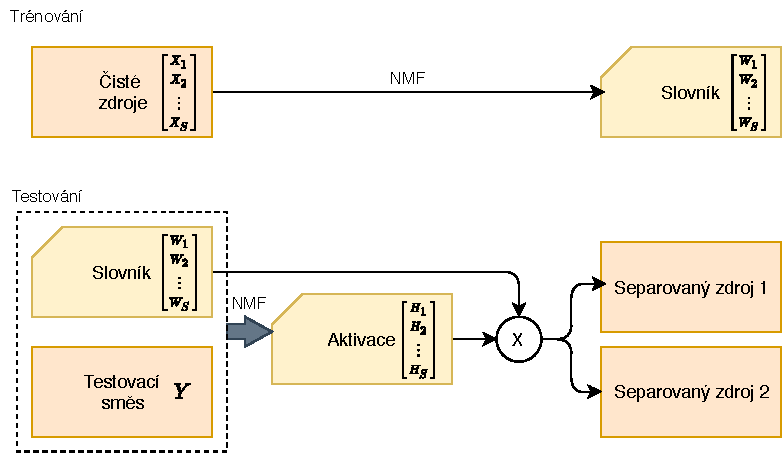
\includegraphics[scale=0.9]{obrazky-figures/nmf.pdf}
    \caption{\label{fig:nmf}Znázornění trénovací a testovací fáze. Obrázek byl inspirován~\cite{speechseparation}.}
\end{figure}

Stejně jako metoda CASA, i tato má mnoho nevýhod, které omezují její použití pro řešení reálných problémů separace.



\subsection{Hluboké neuronové sítě}
Nejlépe si při řešení problému separace mluvčích vedou postupy založené na hlubokém učení a neuronových sítích. Takové modely jsou nejefektivnější, jsou--li definovány jako problémy učení s~učitelem. Podle definice~\ref{equ:definiceseparace}, je cílem separace rekonstruovat původní zdroj signálu.

Metody většinou převáděly směs do časově--frekvenční (T--F) reprezentace znázorněné na obrázku~\ref{fig:spektrum} pomocí short--time Fourier transform (STFT). Tato reprezentace $Y(t,f)$ sloužila pro rekonstrukci každého zdroje $X_s(t,f)$ v~T--F doméně pro každý časový bod $t$ a frekvenci $f$. Vzhledem k~nekonečnému počtu kombinací zdrojových signálů, ze kterých by se dala poskládat původní směs, je nutné naučit model vlastnosti signálů z~trénovacího datasetu a odstranit tak nemožné kombinace~\cite{speechseparation}.

Takový problém lze formulovat jako mnoha--třídový regresní problém. Máme--li vstupní příznak $Y(t,f)$ směsi mluvčích, model se bude učit predikovat individuální tok příznaků $X_s(t,f)$ pomocí vhodného trénovacího datasetu. Později se ukázalo, že se lepších výsledků dosáhne, bude--li model odhadovat množinu masek $M_s(t,f)$ pro každý ze zdrojů, místo přímého odhadu spektra $X_s(t,f)$ a ty pak použít k~rekonstrukci spektra $X_s(t,f)$ jako $X_s = M_s \circ Y$, kde $\circ$ je násobení po prvcích. Masky jsou invariantní vůči proměnným vlastnostem vstupních dat a jejich správný odhad je důležitým faktorem pro kvalitu separace~\cite{speechseparation}.

% https://link-springer-com.ezproxy.lib.vutbr.cz/content/pdf/10.1631/FITEE.1700814.pdf

\begin{figure}[H]
    \centering
    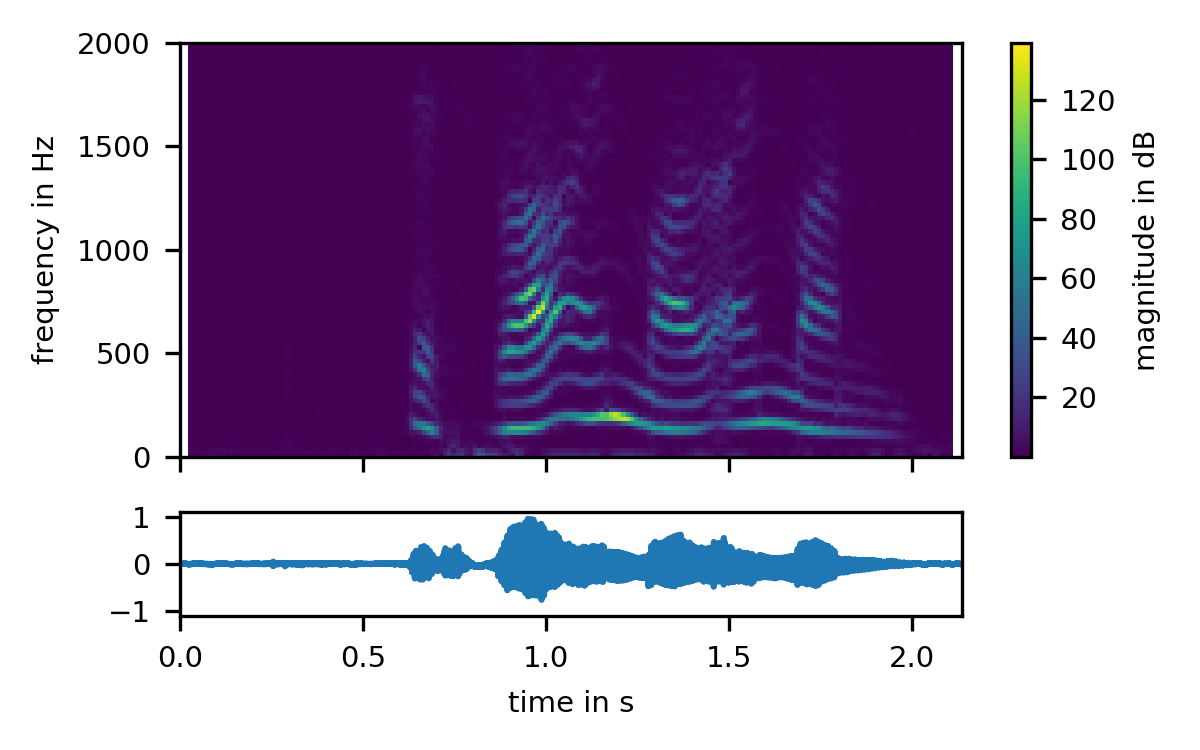
\includegraphics[scale=1.15]{obrazky-figures/spektrum.png}
    \caption{\label{fig:spektrum}Ukázka nahrávky řeči a korespondujícího spektrogramu, na němž jsou zobrazeny frekvence (osa $y$) z~nahrávky řeči v~čase (osa $x$). Zvuk se na spektrogram (T--F reprezentaci) převádí pomocí operace short--time Fourier transform (STFT). Obrázek převzat z~\cite{speech-spectrogram}.}
\end{figure}


Vzniklo mnoho dalších přístupů založených na hlubokém učení. Jeden z~nich ukázal, že pro separaci mluvčích není T--F doména optimální. Architektura TasNet~\cite{luo2018convtasnet}, na kterou se tato práce zaměřuje a je popsána v~kapitole~\ref{tasnet}, převádí vstupní směs na nezápornou reprezentaci a separaci provádí v~časové doméně s~velmi dobrými výsledky.


\section{Vyhodnocovací metriky}
Pro vyhodnocení kvality separace se používají různé metriky. Jejich volba závisí na řešeném problému. Jejich výpočet probíhá na testovacím datasetu. Nejčastěji používané metriky pro měření kvality separace jsou metriky pro vyhodnocování slepé separace zdrojů (BSS), dále short-time objective intelligibility (STOI) a procentuální vyhodnocení kvality řeči (PESQ). Metriky pro BSS jsou source--to--distortion ratio (SDR), signal--to--inference ratio (SIR) a signal--to--artifacts ratio (SAR).


\subsection{Source to distortion ratio}
SDR~\cite{vincent-inria-00544230} je jedna z~nejznámějších metrik pro měření kvality separace mluvčích. Hodnota je udávána v~decibelech (dB). Na výstupu separačního algoritmu se může nacházet rušení, které lze kategorizovat jako inference a artefakty. 

Inference odkazuje na přetrvávající podíl druhého zdroje na separované nahrávce prvního zdroje. SIR je tedy metrika zachycující schopnost algoritmu odstranit ostatní zdroje a zachovat pouze ten požadovaný.

Během separace může algoritmus do separovaných nahrávek zanést artefakty, které se mohou projevovat jako rušení či zvuky, které na původní nahrávce nebyly. SAR je metrika zachycující schopnost algoritmu separovat nahrávky bez toho, aby do nich zanesl nechtěné artefakty~\cite{venkataramani2018performance}.

Metriky SIR a SAR lze zkombinovat do jediné metriky SDR, která udává celkovou kvalitu separace. 

Hodnota SDR se vypočítá jako 
\begin{equation}
  SDR = 10*log_{10}\frac{\|s_{target}\|^2}{\|e_{interf} + e_{noise} + e_{artif}\|^2}
\end{equation}

Hodnoty $e_{interf}$, $e_{noise}$ a $e_{artif}$ udávají chybu inference, hluku a artefaktů. $s_{target} = f(s_j)$ je verze původního zdroje $s_j$, který je obohacen o~dovolenou hladinou rušení $f \in \mathcal{F}$. Metrika je počítána pro každý odhadnutý zdroj $\hat{s_j}$ tak, že ten je porovnán s~referenčním zdrojem $s_j$. V~prvním kroku je dekomponován zdroj $\hat{s_j}$ jako součet $s_{target} + e_{interf} + e_{noise} + e_{artif}$. Ve druhém kroku jsou vypočítány poměry energie, které jsou potřeba při vyhodnocení relativního zastoupení těchto čtyř složek. Je--li při výpočtu porovnáván $\hat{s_j}$ se všemi ostatními zdroji $s_j'$, tak je jako finální vybrána taková hodnota, která během porovnávání dávala nejlepší výsledek. Porovnávat lze buď celý signál, nebo pouze jeho segmenty~\cite{vincent-inria-00544230}. V~této práci je pro výpočet SDR používána knihovna $\texttt{mir\_eval}$~\cite{mir-eval}.


% \cite{vincent-inria-00544230
% \url{https://hal.inria.fr/inria-00544230/PDF/vincent_TASLP06bis.pdf}

% \cite{sdr-pesq-optimization}
% https://arxiv.org/abs/1901.09146


% neco o si-sdr
%http://www.jonathanleroux.org/pdf/LeRoux2019ICASSP05sdr.pdf


\subsection{Perceptual evaluation of speech quality}
Procentuální vyhodnocení kvality řeči (PESQ)~\cite{pesq-itut} je standardizovaná objektivní metoda pro vyhodnocování kvality řeči na end--to--end síti. PESQ byla vyvinuta pro předpověď subjektivního skóre \textit{mean opinion score} (MOS), kde posluchač hodnotil kvalitu připojení (řeči) jednou z~pěti možností (\uv{bad}, \uv{poor}, \uv{fair}, \uv{good}, \uv{excellent}). Těmto možnostem odpovídaly číselné hodnoty $1$ až $5$, které pak byly zprůměrovány, což nakonec byla finální hodnota MOS.

Hodnota PESQ se pohybuje od $-0.5$ do $4.5$ s~tím, že vyšší hodnota znamená lepší procentuální kvalitu~\cite{sdr-pesq-optimization}. Hodnota je určena na základě porovnání originálního signálu a přeneseného signálu skrze komunikační systém. Lze ho ale aplikovat i pro vyhodnocení separace mluvčích, kde referenční nahrávka je porovnána s~nahrávkou, která byla vyprodukována neuronovou sítí.
%http://wireless.feld.cvut.cz/mesaqin2002/full09.pdf

% http://citeseerx.ist.psu.edu/viewdoc/download?doi=10.1.1.5.9136&rep=rep1&type=pdf
%nebo 
% https://arxiv.org/abs/1901.09146
%  \cite{sdr-pesq-optimization}
%dobrej search: https://www.google.com/search?client=firefox-b-d&q=how+pesq+is+calculated

% http://rfmw.em.keysight.com/rfcomms/refdocs/wcdma/wcdma_meas_pesq_desc.html
% https://www.ncbi.nlm.nih.gov/pmc/articles/PMC4452133/



\subsection{Short--time objective intelligibility}
Short--time objective intelligibility (STOI)~\cite{taal-stoi} je metrika založená na hodnotě korelačního koeficientu mezi časově--frekvenčním spektrem referenčního a odhadnutého signálu řeči v~krátkých překrývajících se segmentech~\cite{5713237}. Spektrum čisté a separované nahrávky je získáno pomocí short--time Fourier transform (STFT).

Oba signály jsou dekomponovány pomocí $\frac{1}{3}$--oktávových filtrů pomocí STFT, následně segmentovány na krátké úseky s~$50\%$ překrytím, normalizovány, klipnuty a nakonec porovnány průměry hodnot korelačních koeficientů~\cite{taal-stoi}. Hodnota STOI se pohybuje v~rozmezí $0$ a $1$, korespondující s~procentuální úspěšností, což znamená, že čím vyšší hodnota, tím lepší výsledek.

% Kniha: https://books.google.cz/books?id=ib9ODwAAQBAJ&pg=PA215&lpg=PA215&dq=what+gives+value+of+stoi+in+good+speech&source=bl&ots=14SyU3Hc95&sig=ACfU3U3kMNnhD5fqdunpK2VJ3QRPNHrWTA&hl=en&sa=X&ved=2ahUKEwiQ2ML5gsPqAhUrRBUIHQfOB2wQ6AEwA3oECAgQAQ#v=onepage&q=what%20gives%20value%20of%20stoi%20in%20good%20speech&f=false
% http://citeseerx.ist.psu.edu/viewdoc/download?doi=10.1.1.696.995&rep=rep1&type=pdf
% https://ieeexplore.ieee.org/document/5495701
% https://www.ncbi.nlm.nih.gov/pmc/articles/PMC4452133/




%----------------------------------------------------------------------------------------------------------------------------------------------------------------------
%----------------------------------------------------------------------------------------------------------------------------------------------------------------------
\chapter{Neuronové sítě}
\label{neuronovky}
V~dnešní době zažívají neuronové sítě díky výkonnosti počítačů velký rozmach. Jejich využití prostupuje skrze mnohé vědní obory a dokáží řešit celou řadu problémů, ve kterých dosahují výborných výsledků, které zdaleka předčily dosavadní postupy. 

Neuronové sítě (\textit{artificial neural networks}) jsou výpočetní model, který je inspirovaný strukturou lidského mozku, ve kterém je obrovské množství propojených a komunikujících neuronů. Ty se skládají ze vstupních dendridů, výstupních axonů a samotného těla neuronu. Na základě vnitřního potenciálu a vstupních hodnot je po přesažení prahové hodnoty neuron vybuzen a je vyslán signál na výstupní axon. Signál je nakonec předán dalším neuronům skrze jejich vstupní dendridy~\cite{mitdeeplearning_small}.

Účelem neuronové sítě je naučit se plnit zadanou úlohu. Rozdíl oproti běžným algoritmům je ale ten, že způsob, jakým síť má problém řešit, není explicitně naprogramován, ale je postupně naučen. Základní způsoby učení jsou s~učitelem (\textit{supervised}) a bez učitele (\textit{unsupervised}). 

\textbf{Učení s~učitelem}, pod které spadá i tato práce, spočívá v~mapování vstupních dat na data výstupní na základě vzorových příkladů dvojic vstup--výstup. Množině takových dvojic se říká trénovací dataset.

Mezi problémy, které se dají řešit neuronovými sítěmi patří klasifikační a regresní problémy. Konkrétní příklad z~oblasti klasifikace může být rozpoznávání objektů na obraze, psaného písma nebo detekce obličejů na videu, ale i mnohé aplikace ve zpracování řeči. Problém separace mluvčích, který spadá do zpracování řeči, se dá klasifikovat jako mnoho--třídový regresní problém.

Upravovat samotnou strukturu a chování neuronové sítě lze pomocí jejích hyperparametrů, což jsou parametry určující nastavení neuronové sítě a trénovacího algoritmu. Tyto parametry musí být určeny před začátkem trénování a většinu nelze později měnit. Mohou určovat kapacitu modelu, velikost záběrného pole, velikost filtrů, ale i regulovat samotný proces učení nastavením počtu epoch, po které se model má učit, nebo také počet dat předaný v~jedné dávce (tzv. \textit{minibatches}) během učení sítě.


\section{Organizace dopředných sítí}
Dopředná neuronová síť (feed forward network, či multi layer perceptron -- MLP), zobrazená na obrázku~\ref{fig:mlp}, je typ umělých neuronových sítí, kde se nevyskytují cykly ve výpočetním grafu, tedy zpětná propojení vrstev. Informace se pohybuje pouze jedním směrem, od vstupní vrstvy přes skryté vrstvy až po vrstvu výstupní. Sítě, které obsahují cykly, se nazývají rekurentní a pro představu je taková síť znázorněna na obrázku~\ref{fig:recurrentnn}.

\begin{figure}[H]
    \centering
    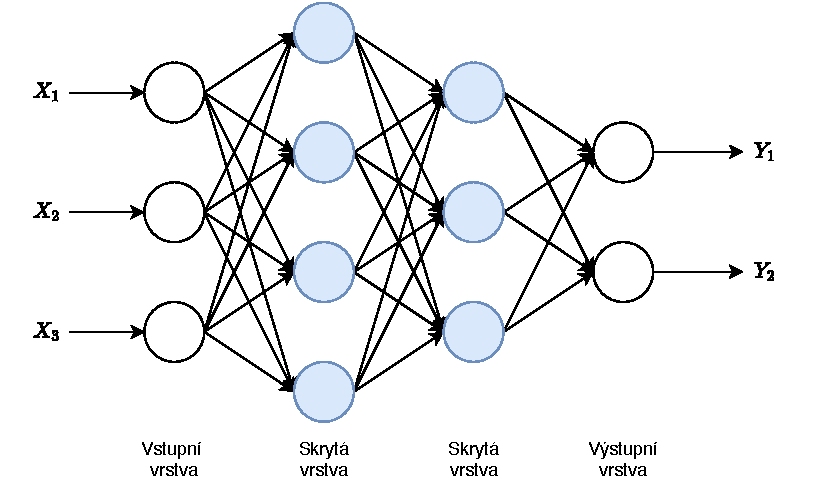
\includegraphics[scale=1.0]{obrazky-figures/mlp.pdf}
    \caption{\label{fig:mlp}Schéma dopředné neuronové sítě, která má 2 skryté vrstvy. Šipky směřují pouze jedním směrem.}
\end{figure}

Struktura neuronové sítě je organizována do vrstev, které se skládají z~neuronů. Dopředná síť je tvořena třemi typy vrstev (viz obrázky~\ref{fig:recurrentnn} a~\ref{fig:mlp}). Vstupní vrstva slouží k~předání hodnot do sítě, ale nijak tyto hodnoty nemodifikuje. Nezměněné jsou zkopírovány do první skryté vrstvy. Následují skryté vrstvy, z~nichž poslední je napojena na výstupní vrstvu. Hodnoty na jejím výstupu mohou představovat třídy, do kterých má být klasifikován vstup v~případě klasifikátorů, nebo predikce hodnot na základě vstupních dat v~případě regrese. S~počtem jednotlivých vrstev souvisí pojem hloubka sítě, která je rovna počtu všech vrstev neuronové sítě od vstupní až po výstupní vrstvu. Pojem \uv{hluboká neuronová síť} označuje takovou síť, která má dvě nebo více skrytých vrstev. Existuje mnoho typů vrstev, například plně propojené, pooling, s~přeskočením nebo vrstvy konvoluční.

\begin{figure}[H]
    \centering
    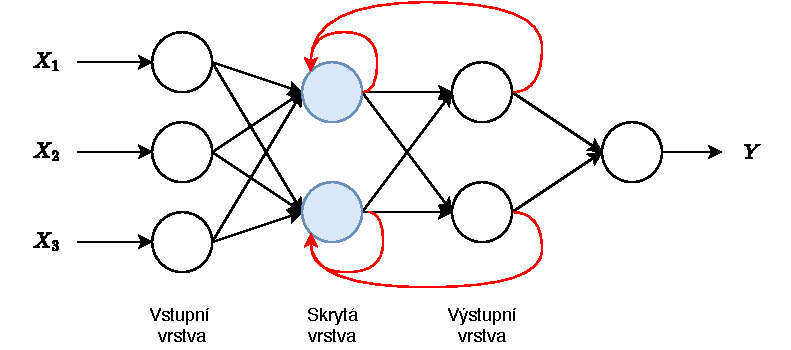
\includegraphics[scale=1.0]{obrazky-figures/feedforward_vs_recurrent.pdf}
    \caption{\label{fig:recurrentnn}Schéma rekurentní neuronové sítě. Lze si všimnout orientace šipek, které směřují i zpět k~předešlým uzlům grafu~\cite{FFandRecNN}.}
\end{figure}


\section{Umělý neuron}
Základní stavební jednotka neuronových sítí je umělý neuron (\textit{artificial neuron}) (viz obrázek \ref{fig:neuron}). Tento model je založen na principu reálných neuronů, které se nacházejí v~organizmech. Umělý neuron obsahuje libovolně mnoho vstupních propojení, přes které se mu předávají data v~podobě vstupního vektoru $\boldsymbol{\overrightarrow{x}} \in \mathbb{R}^N$, kde $\boldsymbol{\overrightarrow{x}} = [x_1, x_2, \dots, x_n], n \in N$. Sám neuron obsahuje hodnotu bias $b \in \mathbb{R}$ a vektor vah $\boldsymbol{\overrightarrow{w}} \in \mathbb{R}^N$, kde $\boldsymbol{\overrightarrow{w}} = [w_1, w_2, \dots, w_n], n \in N$, jenž je upravován během trénování neuronu.

Výstupní hodnota závisí na vstupních datech, aktuálním vnitřním stavu (hodnoty vah a biasu) a na zvolené aktivační funkci. Vstupní hodnoty jsou váhovány, což znamená, že každá vstupní hodnota je vynásobena s~váhou na daném vstupním spojení. S~použitím definovaných vektorů lze napsat, že vstupní vektor je vynásoben s~vektorem vah.

\begin{figure}[H]
    \centering
    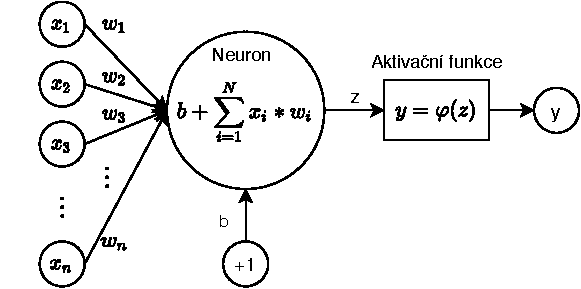
\includegraphics[scale=1.1]{obrazky-figures/perceptron.pdf}
    \caption{\label{fig:neuron}Schéma umělého neuronu.}
\end{figure}

Hodnota bias $b$, která je přičtena k~sumě násobků vah a vstupních hodnot, je prahová hodnota modifikující dobu, kdy se aktivuje neuron a změní svůj výstup. Matematicky to znamená, že s~grafem aktivační funkce horizontálně pohybuje doleva nebo doprava v~závislosti na tom, je-li hodnota biasu pozitivní nebo negativní. V~závislosti na řešeném problému může být žádoucí, aby i hodnota bias byla modifikována během učení společně s~ostatními váhami.

%\begin{figure}[H]
%    \centering
%    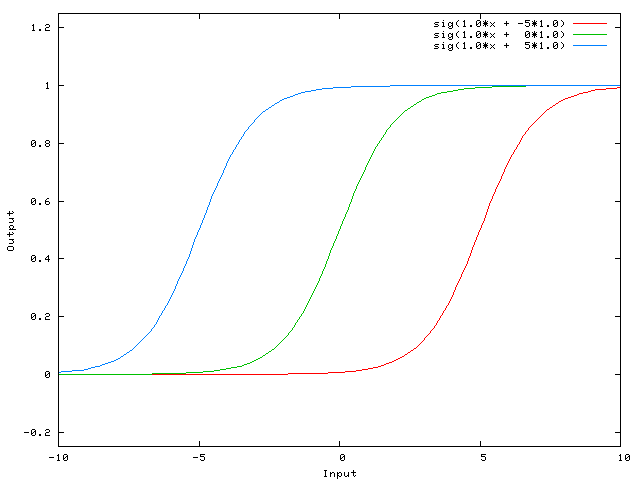
\includegraphics[scale=0.4]{obrazky-figures/bias.png}
%    \caption{\label{fig:bias}Vliv hodnoty bias na aktivační funkci.}
%\end{figure}


Výstup neuronu se vypočítá jako
\begin{equation}
	y = f\Big(b + \sum_{k=1}^N w_kx_k \Big)
\end{equation}
kde $f$ je aktivační funkce, $x_k \in \mathbb{R}$ je vstupní hodnota, $w_k \in \mathbb{R}$ je váha, kterou se vstupní hodnota vynásobí a $b \in \mathbb{R}$ je hodnota bias.


\section{Aktivační funkce}
Aktivační, neboli prahová funkce, určuje výstupní hodnotu neuronu. Funkce se vybírá na základě problému, který se má neuronová síť naučit řešit. Správná volba aktivační funkce vede k~lepší konvergenci učení sítě. Naopak špatná volba může vést ke stále větší odchylce od správného řešení -- může divergovat. Povaha problému může vyžadovat specifické vlastnosti aktivační funkce -- lineární nebo nelineární. Pro nestandardní problémy je obvykle potřeba experimentálně zjistit, která funkce bude nejlépe vyhovovat danému problému. 

Pokud by veškeré aktivační funkce v~modelu byly lineární, tak celkové mapování sítě by bylo omezeno pouze na lineární mapování vstupu na výstup. Reálné problémy ale lineární obvykle nejsou a v~případě pokusu modelovat takovým modelem nelineární vztahy by vedlo k~velice nepřesným výsledkům, který by byl zapříčiněn podučením (\textit{underfitting}), což znamená, že model, který se učí zakódovat nějaký vzor v~datasetu, je příliš jednoduchý. Proto je potřeba zavést do modelu i nelineární aktivační funkce, které tento problém řeší~\cite{mitdeeplearning_small}.

Z~pohledu učení je také důležité, aby aktivační funkce byla diferencovatelná. To umožňuje použití trénovacích metod založených na výpočtu gradientu, jako je algoritmus backpropagation.



\subsection*{Logická sigmoida}
Logická sigmoida je nelineární aktivační funkce používaná v~hlubokém učení, nejčastějí v~dopředných neuronových sítích. Graf funkce má hladký průběh, jak lze vidět na obrázku~\ref{fig:sigmoid}. Je to omezená diferencovatelná funkce, definovaná jako
\begin{equation}
  f(x) = \frac{1}{1+\exp(-x)}
\end{equation}
Používá se na výstupních vrstvách pro predikci výstupu na základě pravděpodobnosti, čehož se využívá při řešení logistických regresních problémů, u~binárních klasifikátorů a dalších oblastí neuronových sítí. Podle~\cite{NEAL199271} je nejčastěji používána v~sítích s~menším počtem vrstev (tzv. shallow networks). Mezi hlavní nevýhody patří ostrý gradient během zpětné propagace, saturace gradientu a pomalá konvergence~\cite{nwankpa2018activation}.

\begin{figure}[H]
    \centering
    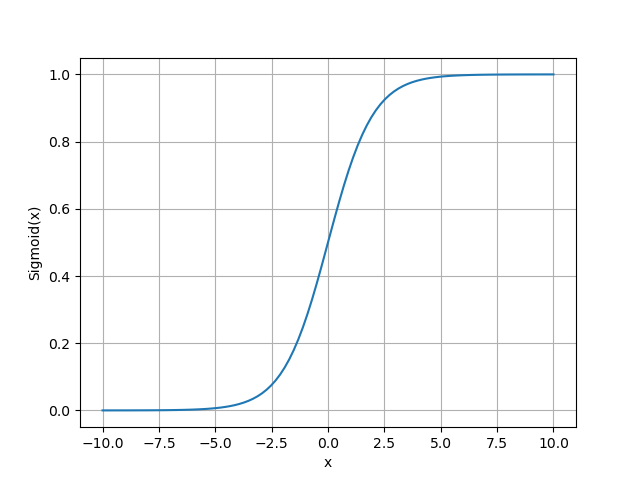
\includegraphics[scale=0.75]{obrazky-figures/sigmoid.png}
    \caption{\label{fig:sigmoid}Graf aktivační funkce sigmoid.}
\end{figure}



\subsection*{Softmax}
Aktivační funkce softmax~\cite{mitdeeplearning}, neboli normalizovaná exponenciální funkce, se často umisťuje na výstupní vrstvy a používá se pro výpočet rozdělení pravděpodobnosti z~vektoru reálných čísel. Výstupem je hodnota v~rozmezí $0$ až $1$, jak zobrazuje graf~\ref{fig:softmax}, na kterém lze vidět, že každá z křivek reprezentuje pravděpodobnost nějaké třídy a jejich součtem v jakémkoli bodě $x$ získáme hodnotu $1$. V~klasifikačních modelech výstup reprezentuje pravděpodobnosti jednotlivých tříd s~tím, že cílová třída má nejvyšší hodnotu pravděpodobnosti~\cite{nwankpa2018activation}. Vypočítá se jako

\begin{equation}
  f(x_i) = \frac{\exp(x_i)}{\sum_j \exp(x_j)}
\end{equation}


\begin{figure}[H]
    \centering
    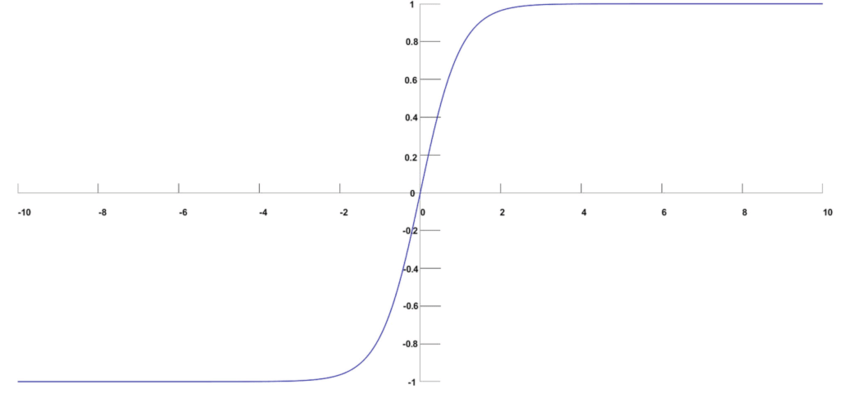
\includegraphics[scale=0.75]{obrazky-figures/softmax.png}
    \caption{\label{fig:softmax}Graf aktivační funkce softmax. Každá křivka reprezentuje pravděpodobnost příslušnosti do nějaké třídy. Graf zobrazuje pravděpodobnostní rozdělení celkem $4$ tříd. Součtem hodnot $y$ v libovolném bodě $x$ získáme hodnotu $1$.}
\end{figure}


\subsection*{Rectified Linear Unit}
\label{relu}
Rectified Linear Unit (ReLU) je nejčastěji používaná aktivační funkce a stojí za nedávnými úspěchy v~oblasti neuronových sítí~\cite{NIPS2012_4824}. Vyžaduje-li síť nějakou nelinearitu, je ReLU pro většinu případů ideální. Její použití zrychluje konvergenci trénovacího procesu a vede k~lepším výsledkům, než u~jednotek používající konvenční sigmoidní aktivační funkce~\cite{40811}. Pro každou zápornou hodnotu $x$ vrací $0$ a pro kladnou hodnotu $x$ vrací tutéž hodnotu $x$, jak jde vidět na grafu~\ref{fig:relu}. ReLU je definována jako 
\begin{equation}
   f(x)=max(0,x)
\end{equation}


\subsection*{Parametric Rectified Linear Unit}
Parametrizovaná ReLU (PReLU)~\cite{he2015delving}, jejíž graf je na obrázku~\ref{fig:prelu}, je nelineární aktivační funkce a je to generičtější varianta funkce ReLU. Používá se v~případě, že chceme produkovat na výstup malý nenulový gradient i v~případě záporné vstupní hodnoty $x$, kdy je vynásobena parametrem $\alpha$. Parametr $\alpha$ reguluje klesání záporné části grafu a adaptivně se učí společně s~ostatními váhami během trénovacího procesu.

Předpis funkce PReLU je definován jako
\begin{equation}
  f(x) =
  \begin{cases}
    x & \text{if } x \geq 0 \\
    {\alpha}x & \text{if } x < 0
  \end{cases}
\end{equation}

V~případě, že je hodnota parametru $\alpha=0$, pak se jedná o~ReLU. Je--li parametr $\alpha = c$, kde $c\in\mathbb{R}$ je malá konstanta (například $c = 0.03$), jedná se o~Leaky ReLU (LReLU) a motivací pro její zavedení bylo vyhnout se nulovému gradientu.


\begin{figure}[H]
    \centering
    \begin{minipage}{0.45\textwidth}
        \centering
        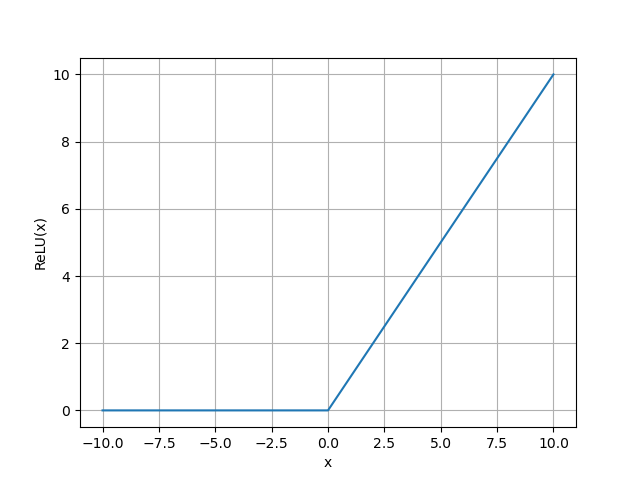
\includegraphics[width=1.00\textwidth]{obrazky-figures/relu.png}
        \caption{\label{fig:relu}Graf aktivační funkce ReLU.}
    \end{minipage}\hfill
    \begin{minipage}{0.45\textwidth}
        \centering
        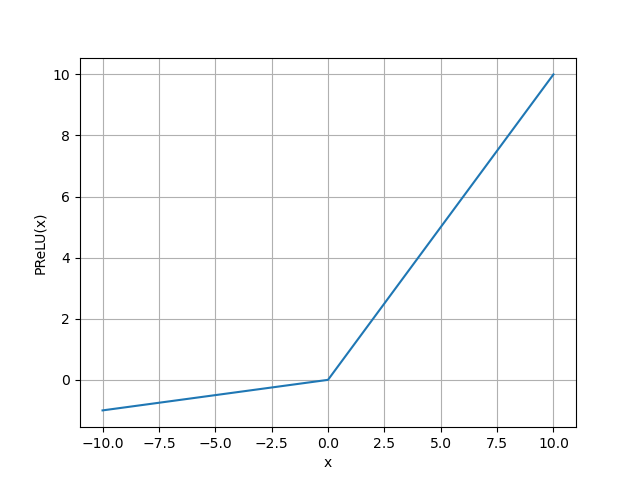
\includegraphics[width=1.00\textwidth]{obrazky-figures/prelu.png}
        \caption{\label{fig:prelu}Graf aktivační funkce PReLU.}
    \end{minipage}
\end{figure}


\section{Konvoluční vrstvy}
Konvoluční neuronová síť (CNN)~\cite{6795724} je typ dopředných neuronových sítí, která obsahuje jednu či více konvolučních vrstev. CNN jsou vhodné pro zpracování dat v~mřížkovitém uspořádání. To může být ve 2--D obrázek ve formě pole pixelů či spektrum nahrávky, nebo vzorky zvukové nahrávky v~čase v~1--D. Konvoluční vrstvy používají místo běžného násobení matic speciální typ lineární operace -- konvoluci.

Diskrétní konvoluce je definována jako
\begin{equation}
   (f \star g)_k = \sum_{i=-\infty}^{\infty} f_i g_{k-i} = \sum_{i=-\infty}^{\infty} f_{k-i} g_{i}
\end{equation}
kde $\star$ je konvoluční operátor, $f$ je funkce signálu, funkce $g$ je konvoluční jádro a $f_i$ a $g_i$ jsou hodnoty funkce na indexu $i$.


Účelem CNN je v~prvních vrstvách sítě extrahovat lokální příznaky ze vstupu. V~pozdějších vrstvách neurony kombinují extrahované lokální příznaky do komplexnějších příznaků (oko, nos), až dokud nezformují v~konečných vrstvách například celý obličej, znak, kočka či jiný objekt, který se síť učí detekovat. V~některých modelech zpracování řeči je zvuk transformován na 2--D spektrogram (viz obrázek \ref{fig:spektrum}) a lze s~ním pracovat stejně, jako při zpracování obrazu.


\begin{figure}[H]
    \centering
    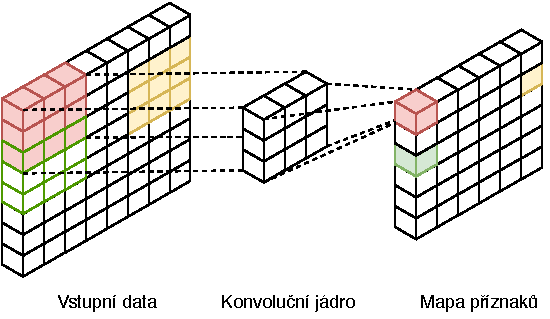
\includegraphics[scale=1.0]{obrazky-figures/convmapping.pdf}
    \caption{\label{fig:convmapping}Průběh konvoluování jádra se vstupními daty a mapování lokálních příznaků na prostor příznaků (feature space), který je výstupem konvoluce. Jádro je postupně aplikováno skrze celý vstup. Je zde také dobře vidět, jak velikost jádra ovlivňuje rozměr výstupních dat. Jádro o~rozměru $3 \times 3$ zmenšilo rozměr vstupních dat o~rozměru $8 \times 8$ na výstupní rozměr $6 \times 6$. Toto chování se dá ovlivnit například zvýšením hodnoty \textit{padding}.}
\end{figure}

Konvoluování jádra přes nějaký vstup (například obrázek či zvuk) je ekvivalentní s~detektorem, který detekuje nějaký lokální příznak. Při aplikaci takového detektoru přes nějaký vstup zaznamenává všechny pozice, kde se příznak nacházel~\cite{mitdeeplearning_small}. Jak vypadá konvoluování a mapování příznaků ilustruje obrázek~\ref{fig:convmapping}.

Během trénování CNN jsou učeny váhy sítě (filtry) k~detekci různých úrovní komplexnosti příznaků. Aby síť dokázala detekovat příznak nezávisle na jeho transformaci (pootočení, převrácení, posuvu), měla by být invariantní. Toho lze docílit tak, že neurony budou sdílet některé váhy (filtry).


Konvoluční operace je definována jako
\begin{equation}
   s[n] = (x \star w)[n]
\end{equation}
kde $x$ jsou vstupní data obvykle ve formě multidimenzionílního pole (tenzoru) a funkce $w$ je konvoluční jádro. Výstupem operace je mapa příznaků. Konvoluční operaci lze definovat i pro vyšší dimenze. Máme--li například 2--D vstupní obrázek, pak i konvoluční jádro bude dvourozměrné. Přestože v~mnoha knihovnách lze nalézt implementovanou operaci konvoluce, často se jedná o~cross--korelaci.


Průběh a chování konvoluce lze řídit hyperparametry \textit{stride}, \textit{padding} a \textit{dilation}. Hodnota stride modifikuje velikost kroku konvolučního jádra. Chování při různých hodnotách lze vidět na obrázku~\ref{fig:conv_stride1} a~\ref{fig:conv_stride2}. 

Hodnota padding určuje, o~kolik se mají rozšířit vstupní data. V~případě malého rozměru konvolučního jádra může dojít k~nechtěné změně rozměrů vstupních dat a proto se tato data po stranách rozšíří na takový rozměr, aby po konvoluci byl výsledný tvar v~požadovaném rozměru. Vyplnění ukazuje obrázek~\ref{fig:conv_padding}.


\begin{figure}[H]
    \centering
    \begin{minipage}{0.45\textwidth}
        \centering
        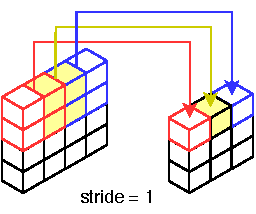
\includegraphics[width=0.7\textwidth]{obrazky-figures/stride1.pdf}
        \caption{\label{fig:conv_stride1}Hodnota stride ovlivňuje konvoluční krok jádra nad zpracovávanými daty. Čím větší hodnota stride, tím menší je výstupní rozměr dat.}
    \end{minipage}\hfill
    \begin{minipage}{0.45\textwidth}
        \centering
        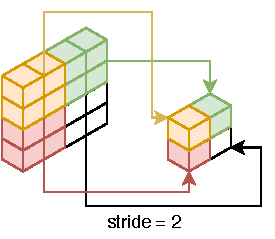
\includegraphics[width=0.7\textwidth]{obrazky-figures/stride2.pdf}
        \caption{\label{fig:conv_stride2}Hodnota kroku ovlivňuje výstupní rozměr dat. Zde je vidět, že při kroku o~velikosti $2$, rozměru jádra $2 \times 2$ a rozměru vstupních dat $4 \times 4$ je výstupní rozměr pouze $2 \times 2$.}
    \end{minipage}
\end{figure}


Hodnota dilation podporuje rozšíření pole působnosti bez ztráty rozlišení nebo pokrytí dat konvolučním jádrem během konvoluční operace (viz obrázek~\ref{fig:conv_dilation} a~\ref{fig:dilation_factor}). Zatímco pole působnosti roste exponenciálně, počet parametrů roste pouze lineárně. Této vlastnosti se využívá například v~temporal convolutional networks (TCN), kde dilatační faktor nabývá hodnot $1, 2, 4, 8, \dots$.

\begin{figure}[H]
    \centering
    \begin{minipage}{0.45\textwidth}
        \centering
        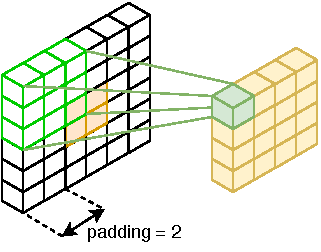
\includegraphics[width=0.8\textwidth]{obrazky-figures/padding.pdf}
        \caption{\label{fig:conv_padding}Nastavením hodnoty padding se zpracovávaná data na okrajích rozšíří o~danou hodnotu a toto rozšíření bude vyplněno nulami či jakoukoli jinou hodnotou.}
    \end{minipage}\hfill
    \begin{minipage}{0.45\textwidth}
        \centering
        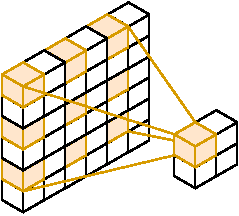
\includegraphics[width=0.7\textwidth]{obrazky-figures/cnndilation.pdf}
        \caption{\label{fig:conv_dilation}Vizualizace hodnoty dilatace upravující pole působnosti.}
    \end{minipage}
\end{figure}

%\begin{figure}[H]
%    \centering
%    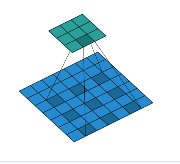
\includegraphics[scale=1.0]{obrazky-figures/cnndilation.png}
%    \caption{\label{fig:conv_dilation}Vizualizace hodnoty dilatace upravující pole působnosti}
%\end{figure}

\begin{figure}[H]
    \centering
    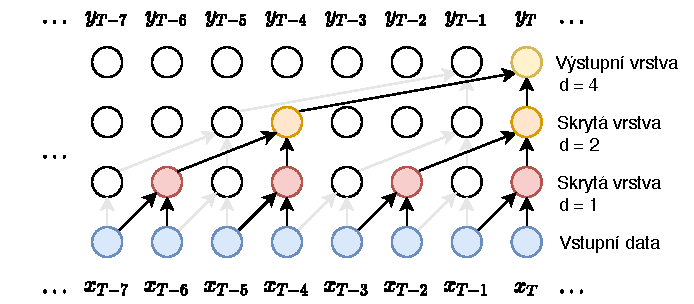
\includegraphics[scale=1.1]{obrazky-figures/causal_dilation.pdf}
    \caption{\label{fig:dilation_factor}Vizualizace časové dilatace na vstupním signálu. Zde je vidět kauzální konfigurace, při které je hodnota $y_T$ počítána pouze z~hodnot v~čase $t \leq T$.}
\end{figure}

Dalším faktorem, který ovlivňuje výpočet, je kauzalita sítě. Tato vlastnost určuje, která data mohou být použita pro výpočet výstupní hodnoty. Kauzální nastavení sítě ilustruje obrázek~\ref{fig:dilation_factor}, zatímco obrázek~\ref{fig:noncausal} ukazuje nekauzální konfiguraci, kde je hodnota $y_T$ počítána i z~hodnot v~čase $t > T$.

\begin{figure}[H]
    \centering
    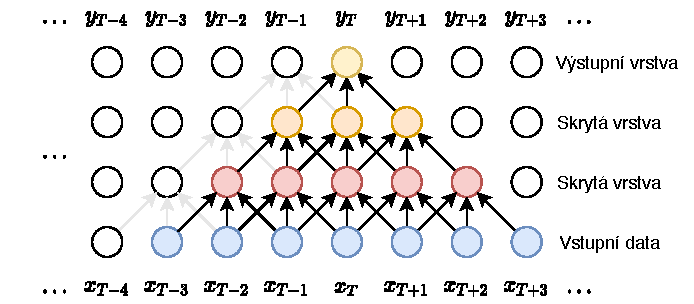
\includegraphics[scale=1.1]{obrazky-figures/non-causal.pdf}
    \caption{\label{fig:noncausal}Nekauzální konfigurace umožňující výpočet hodnoty i z~budoucích dat. Zde není použita časová dilatace (ale mohla by být).}
\end{figure}

\section{Učení neuronových sítí}
Cílem trénování je naučit neuronovou síť vykonávat nějaký úkol. Trénování založené na metodě učení s~učitelem vyžaduje dostatečně velký dataset obsahující dvojice vstup--výstup a obnáší volbu objektivní funkce, kterou se během trénování snažíme minimalizovat. 

Formálně je cílem učení aproximovat nějakou funkci $f^\ast$. Síti je předána vstupní hodnota $x$, pro kterou síť definuje mapování na výstupní hodnotu jako $y = f(x; \theta)$, kde $\theta$ je parametr, který se síť učí tak, aby dosáhla nejlepší aproximace funkce~\cite{mitdeeplearning}.


\subsection{Objektivní funkce}
Objektivní funkce (loss funkce, cost funkce) je funkce, která je během učení minimalizována nebo maximalizována, v~závislosti na konkrétním úkolu a kontextu použití. Tato funkce mapuje událost či hodnoty na reálné číslo reprezentující \uv{cenu}, která je asociována s~touto událostí či hodnotami. Je--li tato funkce použita pro optimalizační problém, pak je cílem hodnotu minimalizovat a funkci se pak říká loss funkce. Výstupní hodnota loss funkce nám udává velikost chyby, která se počítá na základě rozdílu mezi výstupem sítě a odpovídajícími trénovacími daty z~datasetu. Pak platí, že čím menší chyba, tím lépe síť provádí svůj úkol, na který je trénována. Použije--li se hodnota objektivní funkce s~opačným znaménkem, tak lze funkci použít jako hodnotící metriku.


V~rámci učení sítě je žádoucí, aby gradient objektivní funkce byl dostatečně velký (prudký) a předvídatelný. V~takovém případě bude dobře sloužit pro účely trénování. V~případě malého gradientu by funkce saturovala (byla by příliš plochá) a to by mohlo negativně ovlivnit trénování sítě~ \cite{mitdeeplearning}. 

Nejčastěji se pro regresní problémy používají objektivní funkce \textit{Mean Squared Error Loss} a \textit{Mean Absolute Error Loss}.


\subsection*{Mean squared error loss}
Mean squared error loss (MSE) je nejčastěji používaná objektivní funkce při řešení regresních problémů. Vypočítá se jako
\begin{equation}
  MSE = \frac{1}{N}\sum_{i=1}^N(y_i - \hat{y_i})^2
\end{equation}
kde $N$ je počet trénovacích dat v~datasetu, $y_i$ je předpovězená hodnota a $\hat{y_i}$ je odhadnutá hodnota. Vzhledem k~druhé mocnině je výsledek vždy pozitivní nezávisle na znaménku hodnot $y_i$ a $\hat{y_i}$. Druhá mocnina také zajišťuje, že čím větší je rozdíl mezi předpovídanou a aktuální odhadnutou hodnotou, tím více se chyba projeví. 
%Funkce dosahuje L2 regularizace.

%\begin{figure}[H]
%    \centering
%    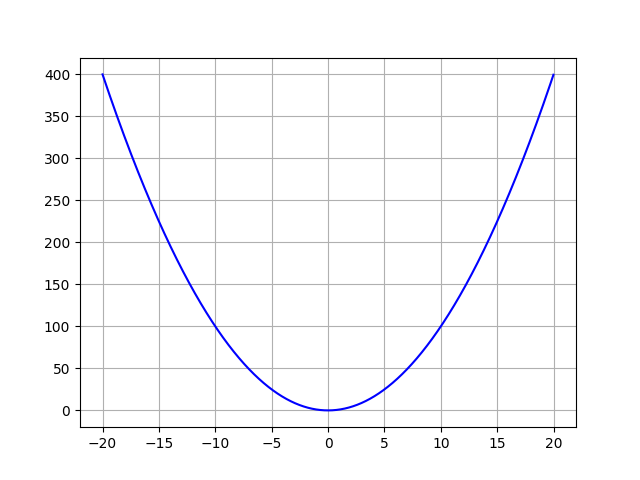
\includegraphics[scale=0.4]{obrazky-figures/mseloss.png}
%    \caption{\label{fig:mseloss}Graf objektivní funkce MSE Loss.}
%\end{figure}


\subsection*{Mean absolute error loss}
Mean absolute error loss (MAE) je velmi podobná objektivní funkce jako MSE, ale s~téměř opačnými vlastnosti. Stejně jako MSE, ani tato funkce nenabývá negativní hodnoty, ale na rozdíl od MSE, která má tuto vlastnost díky druhé mocnině rozdílu, MAE toho dosahuje tak, že rozdíl předpovídané hodnoty $y_j$ a odhadnuté hodnoty $\hat{y_j}$ je uzavřen v~absolutní hodnotě. Vypočítá se jako
\begin{equation}
  MAE = \frac{1}{N}\sum_{j=1}^N|y_j - \hat{y_j}|
\end{equation}

Výhodnou MAE je její lineární průběh, takže se, vzhledem k~lineární závislosti, chyba projeví úměrně, oproti MSE, kde je závislost kvadratická a i menší chyba se projeví více.

Nevýhodou je, že kvůli absolutní povaze není diferencovatelná v~hodnotě $x=0$, což může mít negativní následky pro výpočet gradientu.

%\begin{figure}[H]
%    \centering
%    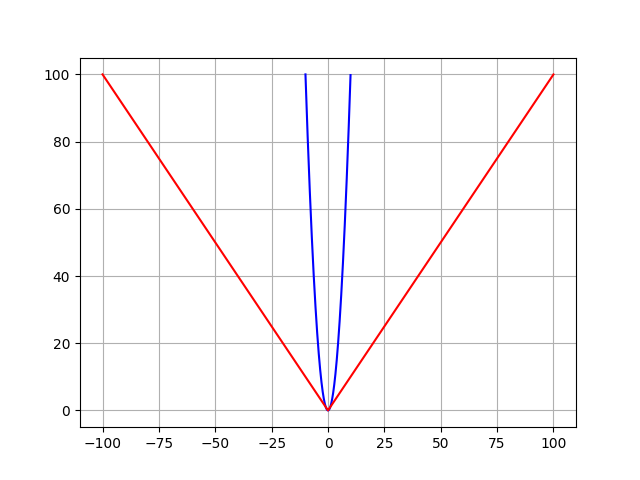
\includegraphics[scale=0.4]{obrazky-figures/maeloss.png}
%    \caption{\label{fig:maeloss}Graf objektivní funkce MAE Loss (červeně).}
%\end{figure}


\subsection{Algoritmus zpětné propagace}
Algoritmus zpětné propagace (backpropagation algorithm) je adaptační algoritmus pro učení neuronových sítí metodou učení s~učitelem. Algoritmus pozpátku prochází neuronovou síťí a na základě hodnoty loss počítá gradient objektivní funkce $J(\theta)$ vzhledem ke všem váhám v~síti. Skalární hodnota loss je výstupem objektivní funkce $J(\theta)$ a gradient této funkce vyjadřuje, jak moc každá váha přispívá k~celkové chybě. Cílem je minimalizovat hodnotu loss. Algoritmus je nejčastěji používán během trénování neuronových sítí, ale obecně ho lze použít pro výpočet jakékoli derivace~\cite{mitdeeplearning_small},~\cite{mitdeeplearning}.

Proces začíná na výstupní vrstvě sítě. Algoritmus zde pro každý neuron spočítá chybový gradient $\delta$ reprezentující citlivost chyby sítě na změnu váhovaného součtu daného neuronu. Tyto gradienty jsou iterativně zpětně propagovány do předchozích vrstev, na základě nichž jsou počítány gradienty neuronů v~předchozích vrstvách, až po vrstvu vstupní. Pro úpravu vah na základě vypočítaných chybových gradientů se obvykle používá algoritmus gradient descent~\cite{mitdeeplearning_small}.


%\cite{web-brilliant}
%https://ml-cheatsheet.readthedocs.io/en/latest/backpropagation.html


\subsection*{Gradient descent}
Gradient descent je iterativní optimalizační algoritmus, definující pravidla pro samotnou úpravu vah v~síti. Je určený pro hledání lokálního minima diferencovatelné objektivní funkce $J(\theta)$, kde $\theta \in \mathbb{R}^d$ reprezentuje učené parametry modelu. Hledání lokálního minima probíhá úpravou parametrů modelu v~opačném směru, než je hodnota gradientu. Výpočet je prováděn postupným pohybem ve směru největšího klesání, které je určeno zápornou hodnotou gradientu. Rychlost pohybu závisí na velikosti kroku, což udává \textit{learning rate}. Správná volba \textit{learning rate} ovlivňuje rychlost, jakou je nalezeno minimum funkce. Při nízké hodnotě bude výsledek přesnější, ale nalezení minima bude výpočetně náročnější, protože v~každém kroku se počítá nová hodnota gradientu. Při větší hodnotě je riziko, že minimum bude přeskočeno~\cite{ruder2016overview}. Obrázek~\ref{fig:gradientdescent} zobrazuje možný průběh algoritmu.
\begin{figure}[H]
    \centering
    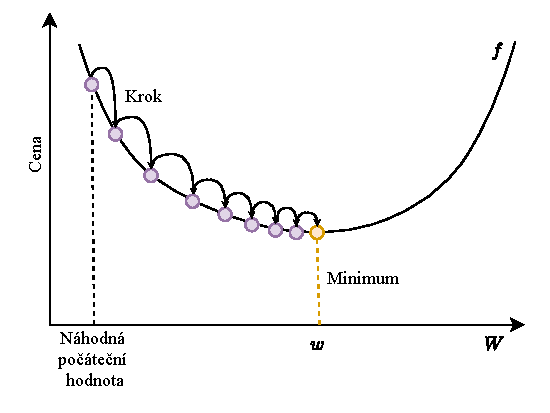
\includegraphics[scale=1.0]{obrazky-figures/gradientdescent.pdf}
    \caption{\label{fig:gradientdescent}Ukázka algoritmu gradient descent při hledání minima dané funkce $f$ postupným přibližováním dle nastavené velikosti kroku. Inspirováno podle~\cite{graddescent}.}
\end{figure}

%\todo{MOZNA sem hodit tu rovnici updatu vah}
% https://ml-cheatsheet.readthedocs.io/en/latest/backpropagation.html


\subsection{Underfitting a generalizace}
Generalizace je vlastnost modelu udávající, jak dobře model pracuje s~dříve neviděnými daty, tedy s~daty, které nebyly použity pro jeho učení. Měří se pomocí testovací chyby. Během učení vzniká učící chyba, která je trénováním postupně minimalizována, ale kvalita modelu je pak měřena na testovacích datech. 

Testovací chyba by ideálně měla být co nejblíže chybě na trénovací sadě. Z~rozdílu mezi těmito chybovými hodnotami se dají diagnostikovat problémy s~naučením sítě -- podučení (\textit{underfitting}) a přeučení(\textit{overfitting}).

\textit{Underfitting} nastane v~případě, že model již nedokáže v~důsledku jeho kapacity zmenšit dostatečně jeho chybovou hodnotu na trénovacím datasetu.

\textit{Overfitting} nastane, když rozdíl mezi trénovací chybou a testovací chybou je příliš velký.

Kapacita je vlastnost modelu určující, kolik se toho dokáže model naučit. V~případě nízké kapacity se model nedokáže naučit všechny příznaky z~trénovacích dat. V~případě vysoké kapacity se mohou přeučit zapamatováním si jejich příznaků a tím sice dosáhnou nízké trénovací chyby, ale špatných výsledků během testování~\cite{mitdeeplearning}. Vliv kapacity na výsledky trénování a testování lze vidět na~\ref{fig:capacity}.
\begin{figure}[H]
    \centering
    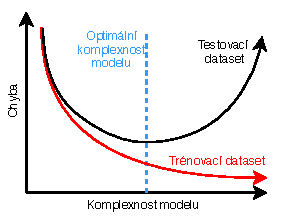
\includegraphics[scale=1.35]{obrazky-figures/capacity_vs_error.pdf}
    \caption{\label{fig:capacity}Vliv kapacity modelu na trénovací a testovací chybu. Obrázek inspirován podle~\cite{trainingvstesterror}.}
\end{figure}

%str 107

Regularizace je souhrn postupů, které říkají, jak modifikovat učící algoritmus tak, aby se zredukovala chyba generalizace, zatímco testovací chyba zůstane stejná~\cite{mitdeeplearning}.

%str 117

\subsection{Reziduální spojení}
Velmi hluboké neuronové sítě přinesly v~mnoha aplikacích velmi dobré výsledky. S~přibývající hloubkou se ale stává její trénování složitější. Jeden z~problémů, který se při učení projevoval, byl explodující a mizející gradient~\cite{279181}. Tento problém byl adresován zavedením normalizačních vrstev~\cite{ioffe2015batch} a počáteční optimalizované inicializace, což dovolilo sítím konvergovat s~využitím \textit{stochastic gradient descent} se zpětnou propagací (\textit{back--propagation})~ \cite{6795724}. Poté se objevil problém degradace, který nebyl zapříčiněn přetrénováním, a způsobil, že s~přibývající hloubkou sítě její přesnost náhle prudce klesla, což indikovalo, že systémy nelze optimalizovat stejným způsobem a přidání dalších vrstev pouze zvýšilo trénovací chybu. Problém degradace lze řešit zakomponováním reziduálních spojení, které je zobrazeno na obrázku \ref{fig:residualconnection}~\cite{he2015deep}.

\begin{figure}[H]
    \centering
    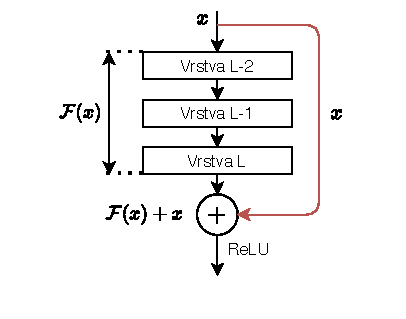
\includegraphics[scale=1.15]{obrazky-figures/residual_connection.pdf}
    \caption{\label{fig:residualconnection}Reziduální spojení mezi vstupem a výstupem stavebního bloku sítě~\cite{he2015deep}.}
\end{figure}

Reziduální spojení, neboli identitní mapování, je zkratka mezi jednou či více vrstvami. Problém mizejícího gradientu řeší tím, že používá aktivace z~předchozí vrstvy, dokud váhy následující vrstvy nejsou naučeny. Spojení lze formulovat jako $\mathcal{F}(x) + x$, kde $\mathcal{F}(x)$ je výsledná hodnota transformace jednotlivými vrstvami a $x$ je původní vstup, který vrstvy přeskočí a následně je sečten s~výstupem $\mathcal{F}(x)$. Výhodou je, že jeho použitím se nezvyšuje počet parametrů ani výpočetní náročnost~\cite{he2015deep},~\cite{zaeemzadeh2018normpreservation}.


\subsection{Význam validační množiny v~trénování}
Většina algoritmů strojového učení má nějakou sadu hyperparametrů, kterou je upravováno chování algoritmu. Hodnoty hyperparametrů obvykle bývají nastavovány ručně ještě před spuštěním procesu učení a hodnota se v~průběhu nemění. Některá nastavení se nicméně mohou stát hyperparametrem a být upravována během trénování, ale není vhodné je měnit na základě výsledku učení na trénovací sadě, protože by mohlo dojít k~přetrénování (\textit{overfitting}). Pro tento případ se použije validační sada, která je odlišná od trénovací sady a síť z ní ještě neviděla nahrávky. Validační sada je zpracována po skončení zpracování trénovací sady a je použita pro monitorování, jak dobře síť generalizuje dosud neviděná data. Na základě výsledků lze následně rozhodnout o úpravě některých hyper--parametrů~\cite{mitdeeplearning}.


%\bigskip
%V~této kapitole byly popsány základní principy neuronových sítí, jejich základní struktura a stavební bloky. V~návaznosti na to byly zmíněny konvoluční sítě, které jsou pro tuto práci stěžejní. Dále byl popsán proces trénování sítí a algoritmy back--propagation a gradient descent. Nakonec byly zmíněny některé oblasti, které se zabývají optimalizacemi sítě, kladoucí si za cíl zlepšit například dobu trénování nebo kvalitu naučení sítě, což může mít za následek lepší výkon sítě při její evaluaci nebo umožnit nasazení ve zdrojově omezeném prostředí.



%----------------------------------------------------------------------------------------------------------------------------------------------------------------------
%----------------------------------------------------------------------------------------------------------------------------------------------------------------------
\chapter{Time--Domain Audio Separation Network}
\label{tasnet}

Tato kapitola vychází z~referenční studie \textbf{TasNet: Surpassing Ideal Time-Frequency Masking for Speech Separation}~\cite{luo2018convtasnet} a popisuje její navrhnuté řešení pro separaci mluvčích v~časové doméně.

Přestože metody pro zpracování řeči v~takovém akustickém prostředí, ve kterém se současně prolíná mnoho řečových signálů, v~poslední době zaznamenaly velké zlepšení, stále trpí mnoha nedostatky. Přesnost systémů, odezva a nároky na výpočetní výkon jsou u~těchto metod natolik zásadní, že znemožňují nebo velmi omezují jejich nasazení mimo výzkumné prostředí, například v~aplikacích, které by mohly zpracovávat řeč v~reálném čase.

Většina dosavadních postupů byla založena na převodu směsi řečových signálů do časově--frekvenční (T--F) reprezentace (spektrogramu) pomocí short--time Fourier transform (STFT), ale tato reprezentace není optimální pro separaci mluvčích~\cite{speechseparationoverview}.

Pro překonání nedostatků předešlých metod byla navržena architektura fully convolutional time--domain audio separation network (Conv--TasNet), založena na hlubokém učení a konvolučních neuronových sítích. Model prvně použije konvoluční enkodér k~převodu krátkých segmentů směsi mluvčích na odpovídající nezápornou reprezentaci, která je optimalizovaná pro extrakci jednotlivých mluvčích. Samotné separace je docíleno aplikací masek na danou reprezentaci. Masky pro každého mluvčího pro každý segment v~každém časovém kroku jsou odhadnuty v~temporal convolutional network (TCN)~\cite{lea2016temporal},~\cite{bai2018empirical}. TCN je tvořena opakující se posloupností konvolučních bloků se zvyšující se časovou dilatací. Po aplikaci masek jsou separovaní mluvčí rekonstruováni lineárním dekodérem. Tuto posloupnost operací zobrazuje zjednodušený obrázek \ref{fig:tasnet-pipe}. Dále v~kapitole budou jednotlivé části popsány detailněji.

\begin{figure}[H]
    \centering
    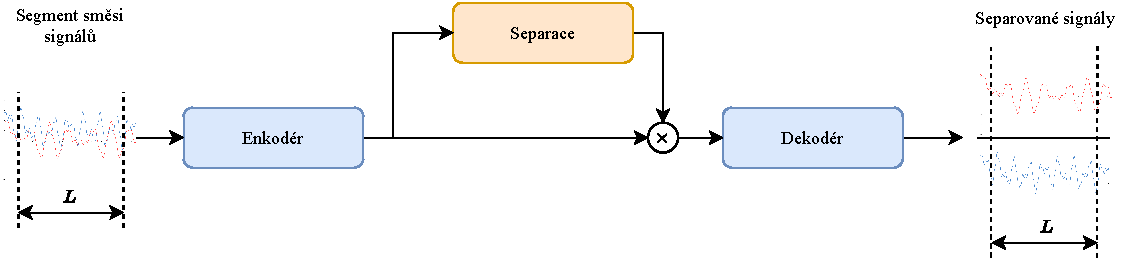
\includegraphics[scale=0.8]{obrazky-figures/tasnet-pipe.pdf}
    \caption{\label{fig:tasnet-pipe}Schéma architektury TasNet.}
\end{figure}


\section{Konvoluční auto--enkodér}
Konvoluční auto--enkodér převádí vstupní segmenty nahrávky na nezápornou reprezentaci a následně zase zpět z~reprezentace na původní nahrávku, jak ukazuje obrázek~\ref{fig:tasnet-autoenkoder}.
\begin{figure}[H]
    \centering
    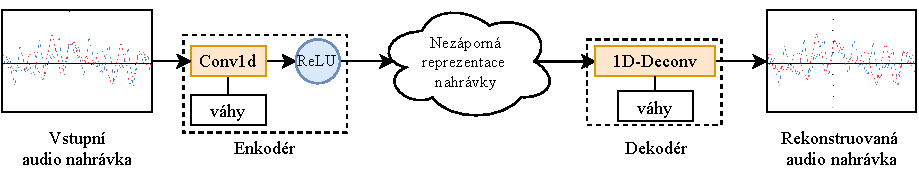
\includegraphics[scale=0.9]{obrazky-figures/autoenkoder.pdf}
    \caption{\label{fig:tasnet-autoenkoder}Schéma konvolučního autoenkodéru.}
\end{figure}


\subsection{Enkódování směsi}
Každý segment směsi o~délce $L$, $\boldsymbol{x_k} \in \mathbb{R}^{1 \times L}$, kde $k = 1, \dots, \frac{T}{L}$, je transformován na nezápornou reprezentaci $\boldsymbol{w} \in \mathbb{R}^{1 \times N}$ pomocí 1--D konvoluční operace jako
\begin{equation}
  	\boldsymbol{w} = ReLU(\boldsymbol{x} \circledast \boldsymbol{U})
\end{equation}
kde $\boldsymbol{U} \in \mathbb{R}^{N \times L}$ obsahuje $N$ vektorů, každý délky $L$, které reprezentují bázové funkce enkodéru. Operace $\circledast$ značí konvoluční operaci. ReLU je nelineární aktivační funkce, která byla blíže popsána v~podkapitole~\ref{relu}.


\subsection{Dekódování extrahovaných mluvčích}
Pro převod z~reprezentace zpět do podoby audio nahrávky slouží lineární dekodér. Pomocí 1--D dekonvoluční operace rekonstruuje původní signál $\boldsymbol{x}$ jako $\boldsymbol{x} \in \mathbb{R}^{1 \times L}$. Tuto operaci lze definovat jako 
\begin{equation}
\label{equ:decoder}
  \boldsymbol{\hat{x}} = \boldsymbol{w}\boldsymbol{V}
\end{equation}
kde každý řádek v~matici $\boldsymbol{V} \in \mathbb{R}^{N \times L}$ představuje jednu bázovou funkci dekodéru s~délkou $L$.

%-------------------------------

\section{Separační modul}
Cílem separačního modulu je najít váhovanou funkci, neboli masku, pro každého zdrojového mluvčího pro každý výstup enkodéru v~každém časovém kroku. Formálně lze zapsat, že cílem je odhadnout $C$ masek $\boldsymbol{m}_i \in \mathbb{R}^{1 \times N}, i = 1, \dots, C$, kde $C$ představuje počet mluvčích ve směsi. Vektory masek $\boldsymbol{m}_i$ mají takové omezení, že $\sum_{i=0}^{C}\boldsymbol{m}_i=1$, kde $1$ je jednotkový vektor v~$\mathbb{R}^{1 \times N}$. Toto omezení garantuje, že rekonstruované zdroje po sečtení zformují původní směs $\boldsymbol{\hat{x}} = \sum_{i=1}^{C}\boldsymbol{\hat{s}}_i$.

Separace je pro každý zdroj provedena vynásobením odpovídající masky $\textbf{m}_i$ s~nezápornou reprezentací (výstupem enkodéru) $w$, jako
\begin{equation}
	\boldsymbol{d_i} = \boldsymbol{w} \odot \boldsymbol{m}_i
\end{equation}
kde $\boldsymbol{d_i} \in \mathbb{R}^{1 \times N}$ je reprezentace každého ze zdrojů a operace $\odot$ je součin po složkách. 

Nakonec jsou reprezentace $\boldsymbol{d_i}$ rekonstruovány zpět na korespondující nahrávky zdrojů $\boldsymbol{\hat{s}}_i, i = 1, \dots, C$ pomocí dekodéru, jak je znázorněno v~\ref{equ:decoder}.


\begin{figure}[H]
    \centering
    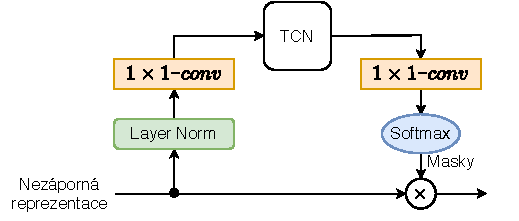
\includegraphics[scale=1.0]{obrazky-figures/separation_module_scheme.pdf}
    \caption{\label{fig:tasnet-separationmodule}Schéma separačního modulu, jehož vstupem je nezáporná reprezentace směsi mluvčích.}
\end{figure}


Na začátku separačního modulu je přidána lineární operace $1 \times 1$--conv jako bottleneck, která určuje počet kanálů na vstupu a výstupu následující sekvence konvolučních bloků. Jak zapadá separační modul do schématu je zobrazeno na obrázku~\ref{fig:tasnet-separationmodule}.

\subsection{Temporal Convolutional Network}
Jádrem separační části je \textit{temporal convolutional network} skládající se z~naskládaných  1--D konvolučních bloků s~časovou dilatací jak lze vidět na obrázku~\ref{fig:tasnet-stacked-resblocks}. Každá vrstva v~TCN obsahuje $X$ konvolučních bloků se zvyšující se časovou dilatací, která se zvyšuje exponenciálně podle počtu bloků a nabývá hodnot $1, 2, 4, \dots, 2^{X-1}$. Taková sekvence bloků je opakována $R$--krát. Exponenciální růst dilatačního faktoru zajišťuje dostatečně velké okno pro využití výhod dlouhých časových závislostí v~signálu řeči. Obrázek~\ref{fig:dilation_factor} zobrazuje rostoucí časovou dilataci na vstupních vzorcích signálu.

Výstup posledního bloku posledního opakování v~TCN je předán $1 \times 1$ konvoluční vrstvě, která má $N \times C$ filtrů a nakonec aktivační funkci softmax k~odhadu $C$ vektorů masek pro každého z~$C$ cílových mluvčích.


\begin{figure}[H]
    \centering
    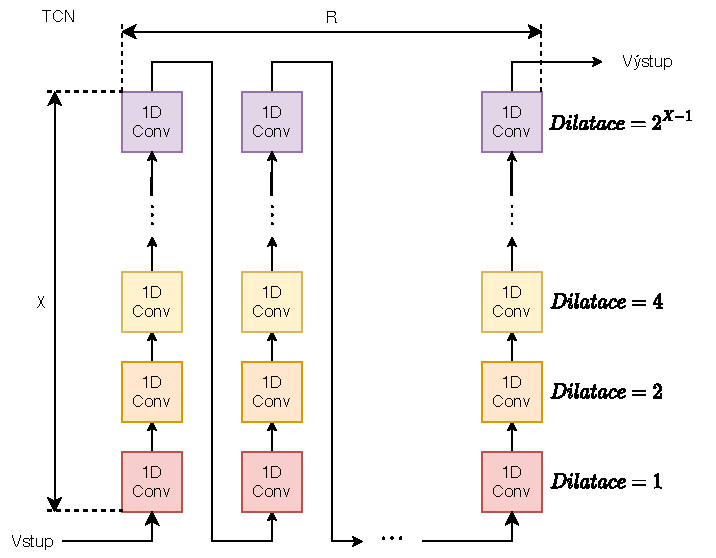
\includegraphics[scale=0.9]{obrazky-figures/stacked_resblocks.pdf}
    \caption{\label{fig:tasnet-stacked-resblocks}Jádro separačního modulu -- naskládané konvoluční bloky s~časovou dilatací odhadující masky na základě nezáporné reprezentace.}
\end{figure}



\subsection{Konvoluční bloky}
Navržená architektura dále nahradila standardní konvoluci uvnitř $1 \times 1$ konvolučních bloků za \textit{depthwise separable convolution} ($S\texttt{-}conv$), která pomáhá snížit počet parametrů a ukázala se jako efektivní ve zpracováni obrazu~\cite{Chollet_2017_CVPR},~\cite{MobileNets}. Konvoluční bloky jsou ve schématu~\ref{fig:tasnet-stacked-resblocks} znázorněny jako \uv{1D~Conv}.

\textit{Depthwise separable convolution} se skládá ze dvou, po sobě jdoucích, operací -- depthwise convolution ($D\texttt{-}conv$) a standardní konvolucí $1 \times 1 \texttt{-}conv$ s~velikostí konvolučního jádra $1$:

\begin{equation}
	D\texttt{-}conv(\boldsymbol{Y}, \boldsymbol{K}) = concat(\boldsymbol{y}_j \circledast \boldsymbol{k}_j), j = 1, \dots, N
\end{equation}

\begin{equation}
	S\texttt{-}conv(\boldsymbol{Y}, \boldsymbol{K}, \boldsymbol{L}) = D\texttt{-}conv(\boldsymbol{Y}, \boldsymbol{K}) \circledast \boldsymbol{L}
\end{equation}

kde $\boldsymbol{Y} \in \mathbb{R}^{G \times M}$ je vstup do $S\texttt{-}conv$, $\boldsymbol{K} \in \mathbb{R}^{G \times P}$ je konvoluční jádro o~velikosti $P$, dále $\boldsymbol{y}_j \in \mathbb{R}^{1 \times M}$ a $\boldsymbol{k}_j \in \mathbb{R}^{1 \times P}$ jsou řádky matic $\boldsymbol{Y}$ a $\boldsymbol{K}$. $\boldsymbol{L} \in \mathbb{R}^{G \times H \times 1}$ je konvoluční jádro o~velikosti 1. Operace $1 \times 1 \texttt{-}conv$ se chová jako plně propojená vrstva a transformuje příznaky do potřebných rozměrů.

\begin{figure}[H]
    \centering
    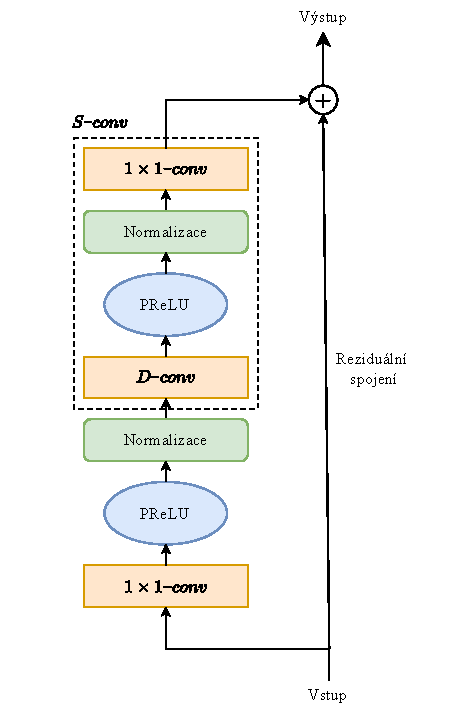
\includegraphics[scale=1.0]{obrazky-figures/conv-res-block.pdf}
    \caption{\label{fig:tasnet-convblock}Jeden konvoluční blok obsahující reziduální spojení mezi vstupem a výstupem. Je zde vidět sekvence operací $D\texttt{-}conv$ a $1 \times 1 \texttt{-}conv$, které dohromady tvoří operaci $S\texttt{-}conv$.}
\end{figure}

V~každém konvolučním bloku jsou operace $1 \times 1 \texttt{-}conv$ a $D\texttt{-}conv$ následovány nelineární aktivační funkcí PReLU~\cite{he2015delving}, která byla popsána v~kapitole \ref{neuronovky}, a normalizační vrstvou. Konvoluční bloky dále obsahují reziduální spojení~\cite{he2015deep} mezi vstupem a výstupem, které výrazně zjednodušuje trénování velmi hlubokých neuronových sítí díky ponechané referenci na vstupní netransformovaná data.


\section{Normalizace}
Při trénování neuronových sítí může docházet k~fenoménu \uv{vnitřní kovariantní posuv} (\textit{internal covariate shift}), kvůli kterému je nutné pečlivě inicializovat parametry a volit menší hodnotu learning rate, což zpomaluje trénování sítě. K~adresování problému slouží zakomponování normalizace do architektury neuronové sítě. Normalizace je aplikována na každý mini--batch trénovacích dat~\cite{ioffe2015batch},~\cite{ba2016layer}.

Konvoluční bloky obsahují normalizační vrstvy, které můžou významně ovlivnit výkon sítě. Ve studii bylo experimentováno s~channel--wise layer normalization (cLN), global layer normalization (gLN) a batch normalization (BN)~\cite{ioffe2015batch}, kterou jsem se rozhodl použít v~mé implementaci.

Metoda cLN je aplikována na vstup separačního modulu pro zajištění invariance při změně měřítka vstupních dat. Tato metoda je vhodná pro použití v~kauzální i nekauzální konfiguraci, je--li použita v~konvolučních blocích. Normalizace cLN je aplikována na každý segment $y_k$. 

Metoda gLN je aplikována globálně na každý příznak na rozměry kanálu i času. Tuto normalizaci lze použít pouze při nekauzální konfiguraci, protože výpočet probíhá na základě celého vstupu.
Při kauzální konfiguraci může být použita také metoda BN.

\bigskip

Jak vypadá kompletní schéma architektury po sestavení a propojení jednotlivých modulů lze vidět na obrázku~\ref{fig:tasnet-modul}. 

\begin{figure}[H]
    \centering
    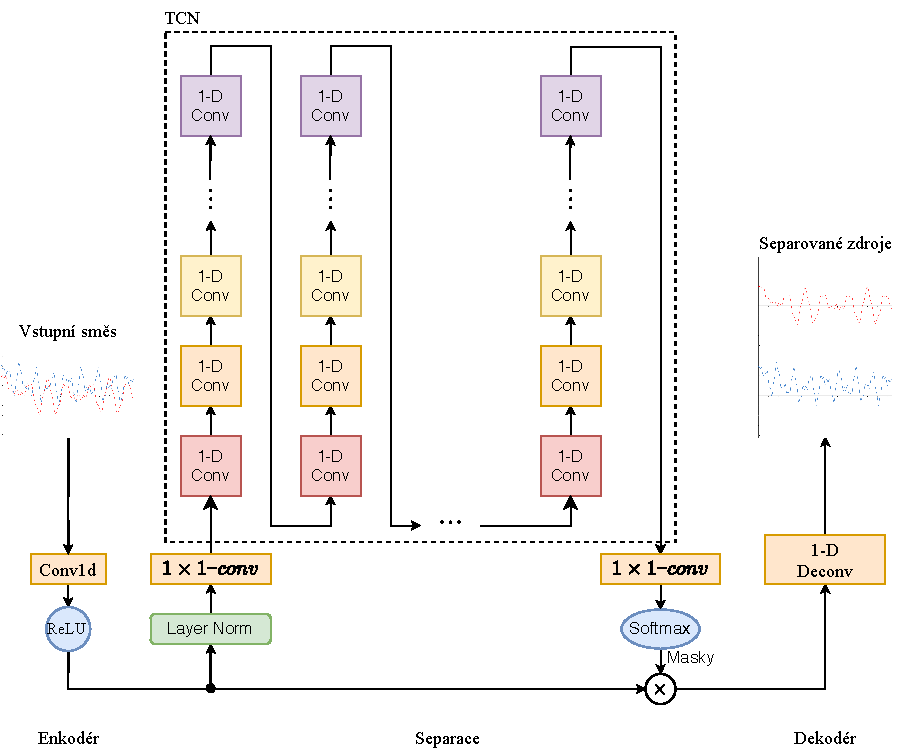
\includegraphics[scale=1.0]{obrazky-figures/tasnet-architecture.pdf}
    \caption{\label{fig:tasnet-modul}Schéma kompletní architektury TasNet.}
\end{figure}


%\bigskip
%V~této kapitole byla popsána navržená architektura Conv--TasNet pro separaci navzájem se překrývajících mluvčích v~časové doméně, skládající se z~konvolučního auto--enkodéru, který převádí vstupní směs mluvčích na nezápornou reprezentaci, ze které je následně v~separačním modulu složeném z~konvolučních bloků se zvyšující se časovou dilatací odhadnuty multiplikativní funkce (tzv. masky) pro každý ze zdrojů. Ty jsou nakonec aplikovány na reprezentaci a výsledek lineárním dekodérem převeden zpět na hlasovou, nyní již separovanou nahrávku.
%----------------------------------------------------------------------------------------------------------------------------------------------------------------------



\chapter{Implementace sítě}
\label{implementace}
Pro implementaci neuronových sítí vzniklo mnoho frameworků jako PyTorch, Tensorflow, Keras a další, které umožňují síť poskládat z~již předdefinovaných modulů. Jejich vlastnosti lze modifikovat dle potřeby pomocí argumentů při jejich instanciaci nebo při jejich použití. Kromě těchto bloků a mnoha dalších možností frameworky obsahují i metody pro práci s~datasety, funkce pro vykreslování grafů a pro matematické operace.

Mým úkolem bylo implementovat neuronovou síť podle architektury TasNet~\cite{luo2018convtasnet} pro separaci mluvčích v~časové doméně. V~rámci zadání jsem si zvolil použít framework s~názvem PyTorch\footnote{\url{https://pytorch.org/}}, který má kvalitní dokumentaci a aktivní uživatelskou základnu. PyTorch funguje nad jazykem Python\footnote{\url{https://www.python.org/}} a v~celé práci používám jeho aktuálně nejnovější verzi (Python~3.8.2). Mimo jiné podporuje práci s~datasety, včetně implementace vlastního nahrávání a manipulace s~daty. Základní jednotkou, se kterou síť pracuje, je tensor. Ve frameworku PyTorch je \texttt{torch.Tensor} třída reprezentující multidimenzionální matici obsahující data jednoho typu. Na tensory jsou převáděna data během načítání datasetu a následně předávána síti ke zpracování. Samotná implementace probíhala na systému Kali linux (4.19.0--kali5--amd64), který je založený na systému Debian. Aplikace byla vyvíjena v~textovém editoru Vim\footnote{\url{https://www.vim.org/}} a byla během implementace spouštěna a testována v~příkazovém procesoru Bash\footnote{\url{https://www.gnu.org/software/bash/}} (Bourne Again SHell) verze 5.0.16. Bash jsem zvolil i pro implementaci některých pomocných skriptů kvůli jednoduchému spouštění z~terminálu a možnostem automatizace některých opakujících se příkazů. Pro správu verzí jsem používal verzovací systém Git\footnote{\url{https://git-scm.com/}}.

Trénování sítě probíhalo z~počátku na CPU \textit{intel i5} mého osobního notebooku \textit{Lenovo Y50--70}, což se ale ukázalo jako naprosto nevhodné vzhledem k~náročnosti výpočtu kvůli nedostatečnému výkonu. Začal jsem tedy používat službu \textit{Google colab}, která poskytuje na omezenou dobu (12 hodin) stroje, které navíc obsahují technologii \textit{cuda}, což mi umožnilo výpočet provádět na GPU, čímž se trénování zrychlilo několikanásobně. Ještě více pomohlo předplacení služby, čímž se mi prodloužila doba, po kterou jsem mohl síť trénovat, na 24~hodin a zvýšila se šance na získání silnějších strojů. Modely byly trénovány na GPU \textit{T80} a \textit{T100} v~závislosti na tom, která z~nich mi zrovna byla přidělena pro dané sezení (\textit{session}). 

Pro vyhodnocování výkonu sítě byly použity metriky SDR, PESQ a STOI. Pro výpočet SDR jsem použil zdrojový kód nacházející se na githubu~\footnote{\url{https://github.com/craffel/mir_eval}}. Metriky PESQ~\footnote{\url{https://github.com/ludlows/python-pesq}} a STOI~\footnote{\url{https://github.com/mpariente/pystoi}} byly nainstalovány pomocí balíkového nástroje pip~\footnote{\url{https://pypi.org/project/pip/}}.

\bigskip

\begin{algorithm}[H]
\caption{\label{alg:zakladnibeh}Zjednodušený algoritmus běhu programu pro trénování sítě.}
\SetNoFillComment
 
 parsování argumentů programu\;
 instanciace modelu TasNet\;
 \If{$args.checkpoint != NULL$}{
	načtení checkpointu\; 
 }
 instanciace třídy SegmentDataset a dataloaderu pro trénovací data\;
 instanciace třídy SegmentDataset a dataloaderu pro validační data\;
 \For{epocha v~args.Epochs}{
  \tcc{trénování}
  loss = 0\;
  \For{směs\_mluvčích z~trénovacího datasetu}{
    \tcc{cyklus načítá z~dataloaderu segmenty nahrávek, které jsou generovány v~třídě SegmentDataset}
  	$odhadovaná\_separace = TasNet(směs\_mluvčích)$\;
  	$loss = sisnr(optimální\_separace, odhadovaná\_separace)$\;
  	propagace chyby a úprava vah\;
  }
  \tcc{validace}
  vypnout gradient\;
  \For{směs\_mluvčích z~validačního datasetu}{
  	$odhadovaná\_separace = TasNet(směs\_mluvčích)$\;
  	$validacni\_loss = sisnr(optimální\_separace, odhadovaná\_separace)$\;
  	\If{hodnota validační loss neklesla potřetí v~řadě}{
		$learning\_rate = learning\_rate / 2$\;
  	}
  }
  na konci epochy uložit checkpoint\;
 }

\end{algorithm}


\section{Implementace tříd a modelu}
Model neuronové sítě byl logicky rozdělen na několik dílčích částí, z~nichž každá je reprezentována jednou třídou. Jednotlivé třídy obsahují metody pro nahrávání a transformaci dat, segmentaci nahrávek a další jsou přímo stavebním blokem neuronové sítě. Některé parametry předané třídám při jejich instanciaci jsou hyperparametry, jejichž hodnoty byly určeny parametry z~příkazové řádky při volání programu. Každá z~tříd bude popsána dále v~textu.


\subsection*{Třídy SegmentDataset a AudioDataset}
Třídy \texttt{SegmentDataset} a \texttt{AudioDataset} slouží pro načítání korespondujících trojic nahrávek směs--zdroj1--zdroj2 z~adresáře, kde je uložen dataset. Nahrávky jsou ve formátu wav a vzorkovány na 8KHz. Třídy tato data dále transformují na tenzory a normalizují na jednotkovou varianci a zero--mean. 

Tyto třídy používají některé pomocné funkce definované v~souboru \texttt{tools.py} pro dorovnání nedostatečně velkých nahrávek ve zpracovávaném mini--batchi nulami na velikost nejdelší z~nich, protože data obsažená v~mini--batchi musejí mít stejnou velikost.

Při spuštění programu jsou nahrány názvy wav souborů do polí, které jsou poté buď náhodně či sekvenčně procházeny a postupně dochází k~načítání trojic nahrávek na aktuálním indexu. 

Obě třídy jsou periodicky volány instancí třídy \texttt{Dataloader}\footnote{\url{https://pytorch.org/docs/stable/data.html\#torch.utils.data.DataLoader}}, která v~cyklu posílá požadavky na data ke zpracování. Rozdíl mezi třídami je ten, že třída \texttt{AudioDataset} předává trojice nahrávek v~původním stavu a délka epochy tak trvá tolik iterací, kolik je nahrávek ve zpracovávaném datasetu a je kvůli tomu používána během testování sítě, kde chceme vyhodnocovat celé nahrávky. Třída \texttt{SegmentDataset} je použita pro trénovací a validační dataset, kde jsou nahrávky rozdělovány na segmenty o~parametrem dané délce a až poté jsou poskytnuty ven. Segmentace je detailně popsána v~podkapitole~\ref{sec:segmentace}.

Po vyčerpání datasetu obě třídy vyvolají vyjímku \texttt{StopIteration}, která je detekována \texttt{Dataloaderem} a ten ukončí cyklus, ve kterém se dataset zpracovával. Tím v~případě trénování končí učení sítě a začíná validace, v~případě validace končí jedna epocha a v~případě testování končí vyhodnocování sítě.


\subsection*{Třída Tasnet}
Třída \texttt{Tasnet.py} reprezentuje model neuronové sítě. Atributy třídy představují jednotlivé vrstvy neuronové sítě. Síť obsahuje konvoluční vrstvy, enkodér, dekodér a \textit{temporal convolutionan network}, která je tvořena sekvencí konvolučních bloků, které jsou rozebrány později. Konvolučním vrstvám jsou nastaveny hodnoty \textit{padding} a \textit{stride}, které ovlivňují chování konvolučních vrstev. V~této třídě jsou také inicializovány váhy (filtry) konvolučních vrstev algoritmem Xavier~\cite{pmlr-v9-glorot10a}. Ve funkci $\texttt{forward()}$, která je volána, když jsou instanci sítě předána data ke zpracování, jsou sekvenčně volány jednotlivé vrstvy. Během zpracování předaných dat je v~této sekvenci vypočítána maska a aplikována na zpracovávanou směs. Tím vzniknou dvě separované nahrávky, které jsou předány na výstup v~podobě tensoru. 


\subsection*{Třída ResBlock}
Třída \texttt{ResBlock} reprezentuje jeden konvoluční blok, který je opakován se zvyšující se dilatací v~\textit{temporal convolutional network} v~separační části určené k~odhadu masek. Podobně jako třída \texttt{Tasnet}, i tato třída obsahuje inicializaci a zřetězení vrstev. V~inicializaci jsou nastaveny hodnoty pro konvoluční operace jako počet konvolučních jader, časová dilatace a počet kanálů. Tyto operace jsou ve funkci $\texttt{forward()}$ zřetězeny do sekvence konvolučních operací a aktivačních funkcí, podle vzorové architektury TasNet. Třída \texttt{ResBlock} je specifická svým residuálním spojením, kde dochází k~rozdělení dat při zpracování, kdy jedna kopie je transformována operacemi v~bloku a na konci sečtena s~daty, které transformacemi neprošly a tento součet je výstupem bloku. Residuální spojení jsou podrobněji popsána v~kapitole~\ref{neuronovky}.


\section{Segmentace nahrávek}
\label{sec:segmentace}
Pro účely trénování sítě byly vstupní nahrávky rozdělovány na segmenty o~délce 4, případně 2 sekund. Délku segmentů $L_s$ lze nastavit přes argument $\texttt{----segment\_length}$ při volání skriptu $\texttt{train.py}$. Tato hodnota reprezentuje jeden z~hyper--parametrů sítě. Výchozí hodnota je 4 sekundy. Při nižších hodnotách se prodlužuje délka trénování, protože se z~jedné vstupní nahrávky o~délce $L$ vygeneruje až $L/L_s$  segmentů a tím narůstá počet dat, který síť musí zpracovat. 

Poslední segment by byl kratší, pokud by délka nahrávky byla kratší než délka segmentu. V~takovém případě je segment doplněn nulami do délky ostatních segmentů jak lze vidět na obrázku~\ref{fig:segmentace_padding}. Toto doplnění je nutné kvůli dávkovému zpracování (\textit{mini--batches}), které neumožňuje rozdílnou délku elementů v~dávce. Pokud je délka nahrávky delší než délka segmentu, tak se poslední segment vezme od konce bez nutnosti ho pak nulami doplňovat. Skládání segmentů do minibatche zobrazuje obrázek~\ref{fig:minibatch_segmentace}. Při vzorkovací frekvenci $f_s = 8000Hz$, obsahují segmenty $f_s * L_s$ vzorků vstupní nahrávky. 

\begin{figure}[H]
    \centering
    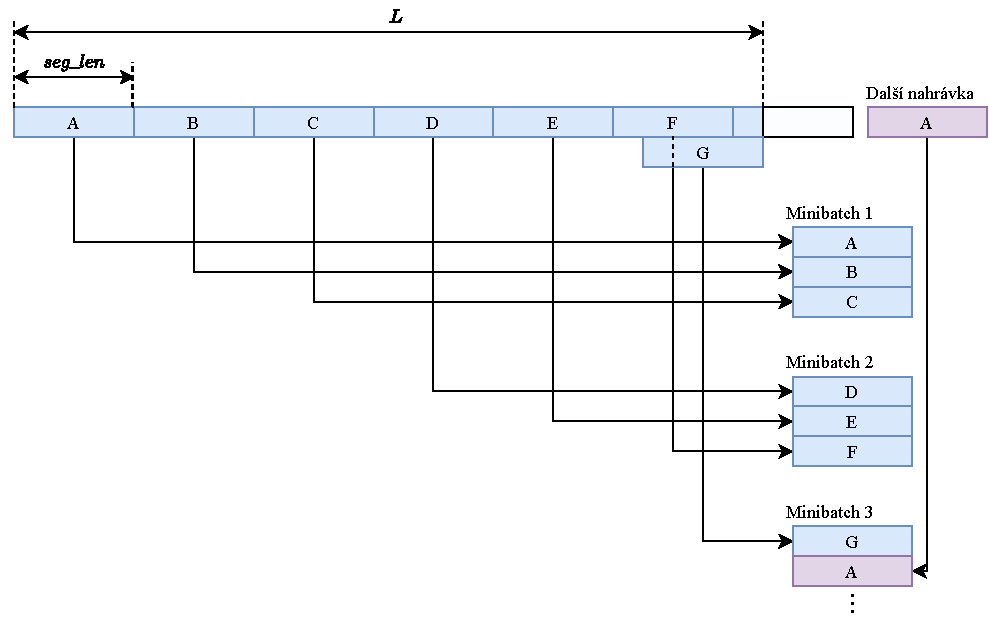
\includegraphics[scale=0.9]{obrazky-figures/minibatch_segmentace.pdf}
    \caption{\label{fig:minibatch_segmentace}Dělení nahrávky na segmenty o~délce \texttt{segment\_len} a jejich následné vkládání do minibatche. Lze si všimnout, že pokud poslední segment není dostatečně dlouhý, tak se vezme od konce nahrávky a jeho počáteční vzorky budou duplicitní s~posledními vzorky předešlého segmentu.}
\end{figure}

\begin{figure}[H]
    \centering
    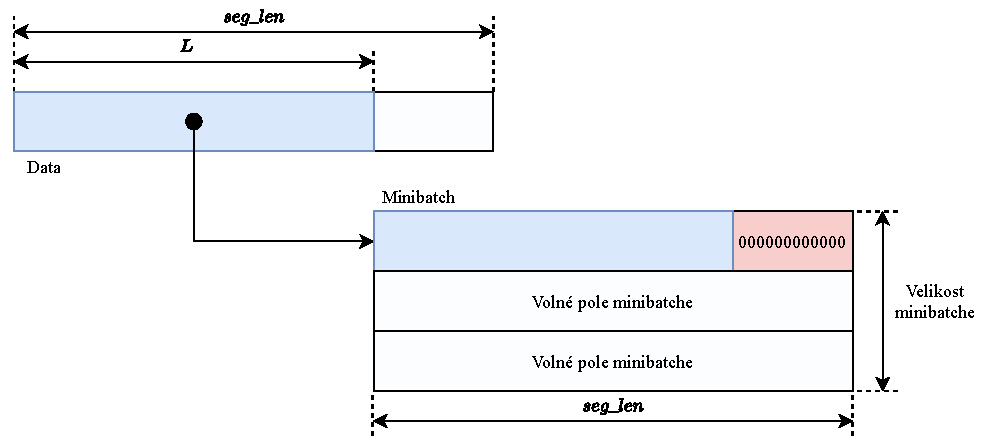
\includegraphics[scale=0.9]{obrazky-figures/minibatch_segmentace_padding.pdf}
    \caption{\label{fig:segmentace_padding}Je--li zpracovávána nahrávka, jejíž délka je kratší než je délka segmentu, je tento segment doplněn z~prava nulami do požadované délky.}
\end{figure}

Algoritmus~\ref{alg:segmentace_nahravek} a obrázek~\ref{fig:generovani_segmentu} zobrazují proces segmentace. Funkce $\texttt{segmentGenerator()}$, která slouží jako generátor, pracuje současně se třemi nahrávkami -- se směsí dvou mluvčích, s~nahrávkou prvního mluvčího a s~nahrávkou druhého mluvčího, které jsou do atributů $\texttt{current\_mixture}$, $\texttt{current\_source1}$ a $\texttt{current\_source2}$ třídy $\texttt{SegmentDataset}$ nahrávány funkcí $\texttt{loadNextAudio()}$ poté, co z~předchozí trojice nahrávek již nelze vygenerovat další segmenty.

\bigskip

\begin{algorithm}[H]
 \caption{\label{alg:segmentace_nahravek}Algoritmus segmenace nahrávek používá výhody Python generátoru, který, na rozdíl od běžných funkcí, po vrácení hodnoty příkazem \texttt{yield} neztrácí svůj vnitřní stav a při jeho dalším zavolání pokračuje tam, kde skončil. V~uvedeném příkladě je znázorněna pouze segmentace nahrávky jednoho mluvčího, ale analogicky se segmentují i nahrávky směsi mluvčích a nahrávky druhého mluvčího. Vizuálně lze sledovat varianty segmentace podle značek A, B, C a D v~komentářích algoritmu na obrázku~\ref{fig:generovani_segmentu}.}

\SetNoFillComment

\SetKwProg{Fn}{Function}{ is}{end}
 \Fn{segmentGenerator() : int[]}{
	 $\texttt{s1\_segment} = \texttt{[]}$\;
	 $\texttt{segptr} = \texttt{0}$\;
	 \While{$\texttt{je dostupná další trojice nahrávek}$}{
		\eIf{$\texttt{current\_mixture\_len} < \texttt{SEGMENT\_LENGTH}$}{
			\tcc{A) aktuální nahrávka je kratší než délka segmentu}
			$\texttt{s1\_segment} = \texttt{current\_source1[:]}$\;
			$\texttt{yield s1\_segment}$\;
		}{
			\tcc{B) aktuální nahrávka je delší než délka segmentu}
			\eIf{$\texttt{segptr} + \texttt{SEGMENT\_LENGTH} < \texttt{current\_mixture\_len}$}{
				\tcc{C) z~aktuální nahrávky vzít segment}				
				$\texttt{s1\_segment} = \texttt{current\_source1[(segptr+SEGMENT\_LENGTH)]}$\;
				$\texttt{segptr} += \texttt{SEGMENT\_LENGTH}$\;
				$\texttt{yield s1\_segment}$\;
			}{
				\tcc{D) nelze již načíst celý segment, takže se vezme od konce}
				$\texttt{start\_index} = \texttt{(current\_mixture\_len - SEGMENT\_LENGTH)}$\;
				$\texttt{s1\_segment} = \texttt{current\_source1[start\_index:current\_mixture\_len]}$\;
				$\texttt{yield s1\_segment}$\;
			}
		}
	}
 }
\end{algorithm}


\begin{figure}[H]
    \centering
    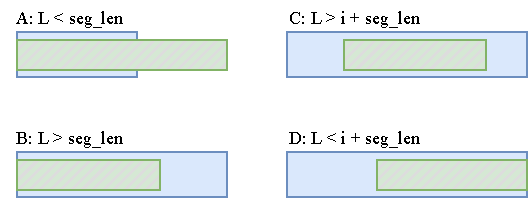
\includegraphics[scale=1.0]{obrazky-figures/segmentation.pdf}
    \caption{\label{fig:generovani_segmentu}Způsob segmentace nahrávek. Obrázek slouží jako doplnění algoritmu~\ref{alg:segmentace_nahravek}. Význam schémat A, B, C a D je označen na odpovídajících pozicích v~komentářích algoritmu. Šrafovaná pole reprezentují vytvářený segment a modrá pole reprezentují data zpracovávaného signálu.}
\end{figure}


Kód segmentace také umožňuje určit délku, o~kterou se segmenty budou překrývat. Této funkcionality je docíleno zavedením proměnné \texttt{overlap}, která obsahuje délku překrytí a při segmentaci je od proměnné \texttt{offset}, který určuje začátek následujícího segmentu, tato hodnota odečtena, jak ukazuje obrázek~\ref{fig:segment_overlap}. Při trénování je překrytí nulové, protože by to zvýšilo počet trénovacích dat jejich částečnou duplikací, což by negativně ovlivnilo délku trénování.

\begin{figure}[H]
    \centering
    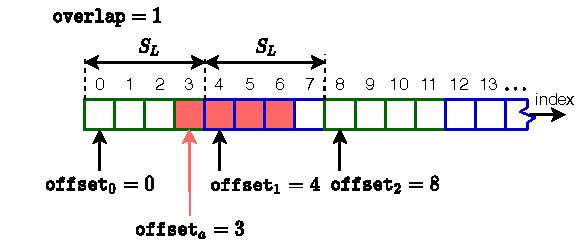
\includegraphics[scale=1.0]{obrazky-figures/segment_overlap.pdf}
    \caption{\label{fig:segment_overlap}Segmentace nahrávek s~nenulovým překrytím. Zde je vidět překrytí (\texttt{overlap}) o~délce $1$. Výsledný \texttt{offset} $n$--tého segmentu se vypočítá jako $\texttt{offset}_n = n*(seg\_len - overlap)$, kde $n = 0, 1, \dots, N$.}
\end{figure}



%\section{Výpočet hodnoty loss za pomoci si--snr}
%\todo{MOZNA}
%\todo{popsat implementaci sisnr a vypocet loss za pomoci cross vypoctu, obrazek}
%
%\begin{figure}[H]
%    \centering
%    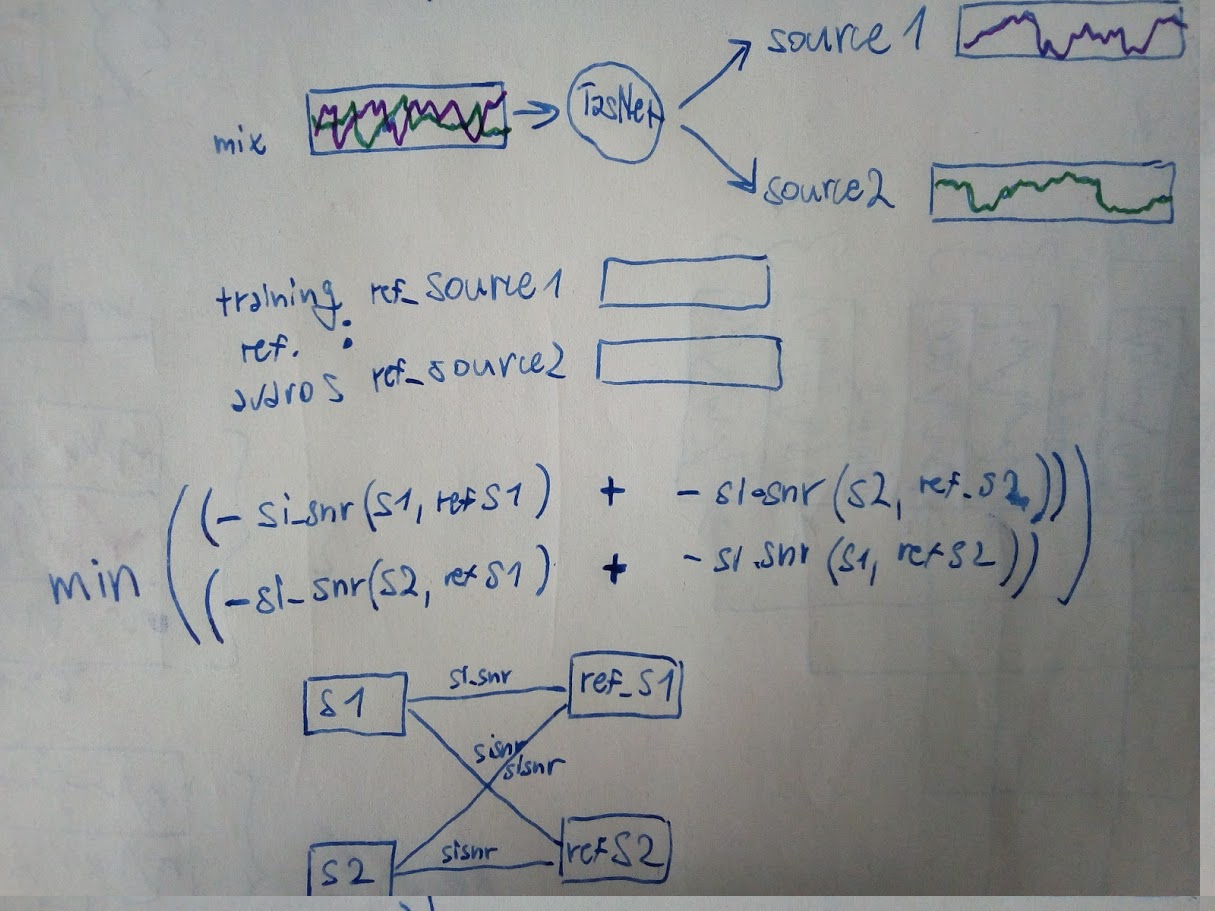
\includegraphics[scale=0.25]{obrazky-figures/sisnr_cross_calculation.jpg}
%    \caption{\label{fig:implementace_loss_sisnr} Implementace a zjištění správné pozice korespondujících nahrávek pro výpočet hodnoty loss}
%\end{figure}
%
% Alg:
% pro kazdou dvojici output--target od 0 do batch_size:
%	vzorecek pro si--sdr loss


\section{Pomocné skripty}
Během implementace se vyskytla potřeba zjednodušit si některé repetetivní úkony a jelikož upřednostňuji práci z~terminálu, tak jsem si pro ně naprogramoval několik skriptů za použití jazyků Python3 a Bash. 

Skript \textbf{\textit{gupload.sh}} pro odesílání zdrojových souborů na \textit{Google Drive}\footnote{\url{https://www.google.com/drive/}}, ze kterého \textit{Google Colab}\footnote{\url{https://colab.research.google.com/notebooks/intro.ipynb}} načítá data a kód, který lze následně po částech spouštět z~grafického rozhraní. K~interakci s~Google Drive jsem použil nástroj \textit{rclone}\footnote{\url{https://rclone.org/}}, který nabízí mnoho operací pro vzdálenou práci s~Google Drive z~terminálu. S~pomocí rclone lze stahovat či nahrávat data, vzdáleně měnit adresářovou strukturu, upravovat soubory a podobně. 

Skript \textbf{\textit{gdownload.sh}} je určený pro snadné stahování dat z~Google Drive pomocí nástroje rsync. Při zavolání stáhne adresář obsahující data z~posledního trénování, nebo adresář, jehož název je předán jako argument skriptu v~příkazové řádce.   
Stažený adresář obsahuje checkpointy, soubory obsahující výstup trénování, soubor obsahující dvojice hodnot \texttt{[zpracováno\_nahrávek, loss]}, které lze jednoduše vykreslit do grafu, a nakonec soubor s~výsledky testování obsahující hodnoty metrik pro testovaný checkpoint.

Dále jsem vytvořil několik jednoduchých skriptů pro rychlé spuštění trénování a testování modelu s~různými přednastavenými parametry. Bylo tak možno mít mezi skripty rozdílné cesty k~adresářům pro účely trénování a ladění chyb nebo třeba nastavení času, po kterém se proces má sám ukončit. Pro spuštění trénování modelu tak lze zavolat skript \textbf{\textit{nntrain.sh}}, pro testování skript \textbf{\textit{nntest.sh}} a pro inferenci (separaci mluvčích na předané nahrávce) skript \textbf{\textit{nninference.sh}}. Skript \textbf{\textit{nninference.sh}} přijímá na svém vstupu směs mluvčích a vyžaduje checkpoint s~naučenou sítí. Jeho výstupem jsou dvě separované nahrávky.


%\bigskip

%Implementace samotného modelu ve frameworku PyTorch nebyla náročná. Vzhledem k~netriviálnímu úkolu jsem musel implementovat některé části, jako třeba segmentace nahrávek, sám. To přineslo mnoho potíží při odstraňování chyb v~samotném modelu. Síť jsem prvně trénoval a ladil na CPU svého notebooku, takže probíhalo velmi pomalu (v~řádu desítek hodin i při nízké velikosti modelu), a některé chyby se objevily až v~průběhu trénování nebo dokonce na jeho konci. Situaci razantně zlepšil přechod na Google Colab, kde jsem síť trénoval na poskytovaných GPU a trénování tak zabralo \todo{"pouze" (opravit uvozovky)} několik hodin, takže se případná chyba objevila dříve, ale i přesto mi lazení sítě zabralo mnoho času. Pro další usnadnění samotné implementace jsem vytvořil několik skriptů, které mi usnadnily spouštění a lazení sítě.



%----------------------------------------------------------------------------------------------------------------------------------------------------------------------


\chapter{Experimenty a vyhodnocení}
\label{experimenty}
Neuronové sítě představují mocný nástroj mnoha využití, který ale musí být naučen, jak danou činnost provádět. Trénování sítí je výpočetně náročný úkol, jehož náročnost se, krom dalších parametrů, může lišit v~závislosti na velikosti datasetu a sítě. Obecně čím větší dataset a rozměr sítě, tím déle trénování trvá. Proto je podstatný výkon stroje, na jakém je síť učena. Je--li k~dispozici výkonný stroj, dá se doba trénování výrazně snížit.

Po dostatečném natrénování probíhá vyhodnocení sítě. Výsledky trénování jsou měřeny metrikami, které se volí na základě problému, který se síť učila řešit. Výsledky testování sítě jsou následně porovnávány v~závislosti na velikosti daného modelu. Velikost modelu je ovlivněna hyper--parametry X, který ovlivňuje počet konvolučních bloků, hyper--parametrem R, který ovlivňuje počet opakování sekvence bloků a velikost segmentace nahrávek při trénování.

Cílem experimentů je zjistit, které z~hyper--parametrů mají největší vliv na kvalitu separace a tedy na výsledky vyhodnocení, a jak moc lze model zmenšit, aby stále dával dostatečně dobré výsledky separace. Kvalita separace je měřena metrikami STOI, SDR a PESQ, které byly popsány v~kapitole~\ref{separace}.


\section{Dataset}
%Dataset je množina dat, na kterých je síť učena a testována. Dataset se dá rozdělit na tři podmnožiny, které jsou navzájem exkluzivní. Trénovací dataset je určen k~trénování sítě a bývá největší. Validační dataset se prochází po zpracování trénovacího datasetu v~průběhu trénování a slouží pro ověření, že hodnota loss na dosud neviděných datech stále klesá a nedochází tak k~přetrénování. Při zpracování tohoto datasetu je síti zabráněno v~učení. Poslední je testovací dataset, na kterém probíhá vyhodnocení sítě, tedy výpočet hodnot jednotlivých metrik. 

Trénování a vyhodnocení modelu proběhlo na množině jednokanálových nahrávek směsí dvou mluvčích. Množina byla vygenerována náhodným výběrem různých mluvčích z~Wall Street Journal (WSJ0)~\cite{DBLP-dataset} a vytvořením směsi mluvčích z~těchto dvou náhodně vybraných nahrávek. Celková délka trénovacích dat je přes $10$ hodin a přes $6$ hodin validačních dat. Testovací data jsou vygenerována z~16ti, doposud neviděných, mluvčích. Nahrávky jsou převzorkovány na 8kHz a během trénování zarovnány na \textit{zero means} a jednotkovou varianci. Skript pro generování datasetu lze nalézt v~\footnote{https://www.merl.com/demos/deep-clustering}.

\begin{figure}[H]
    \centering
    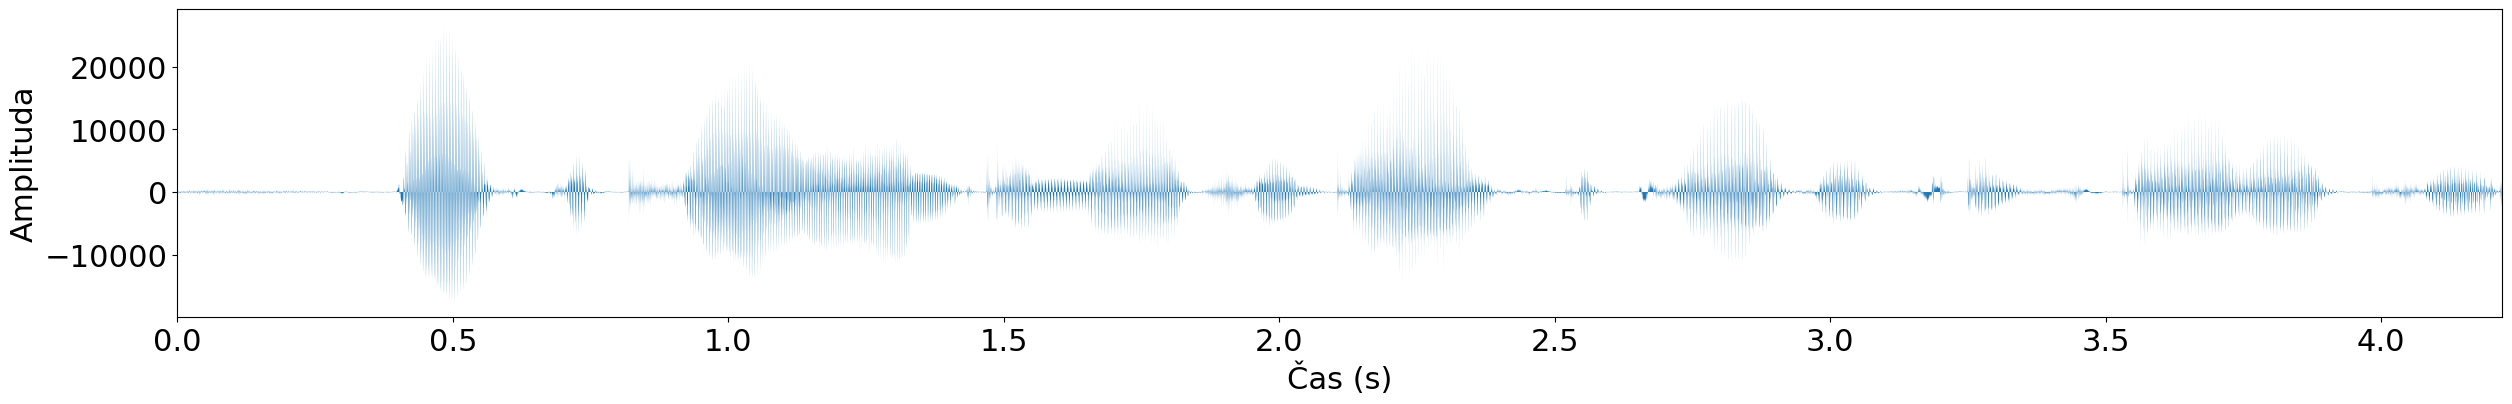
\includegraphics[scale=0.24]{obrazky-figures/s1.png}
    \caption{\label{fig:ref-s1}První mluvčí ze směsi}
\end{figure}

\begin{figure}[H]
    \centering
    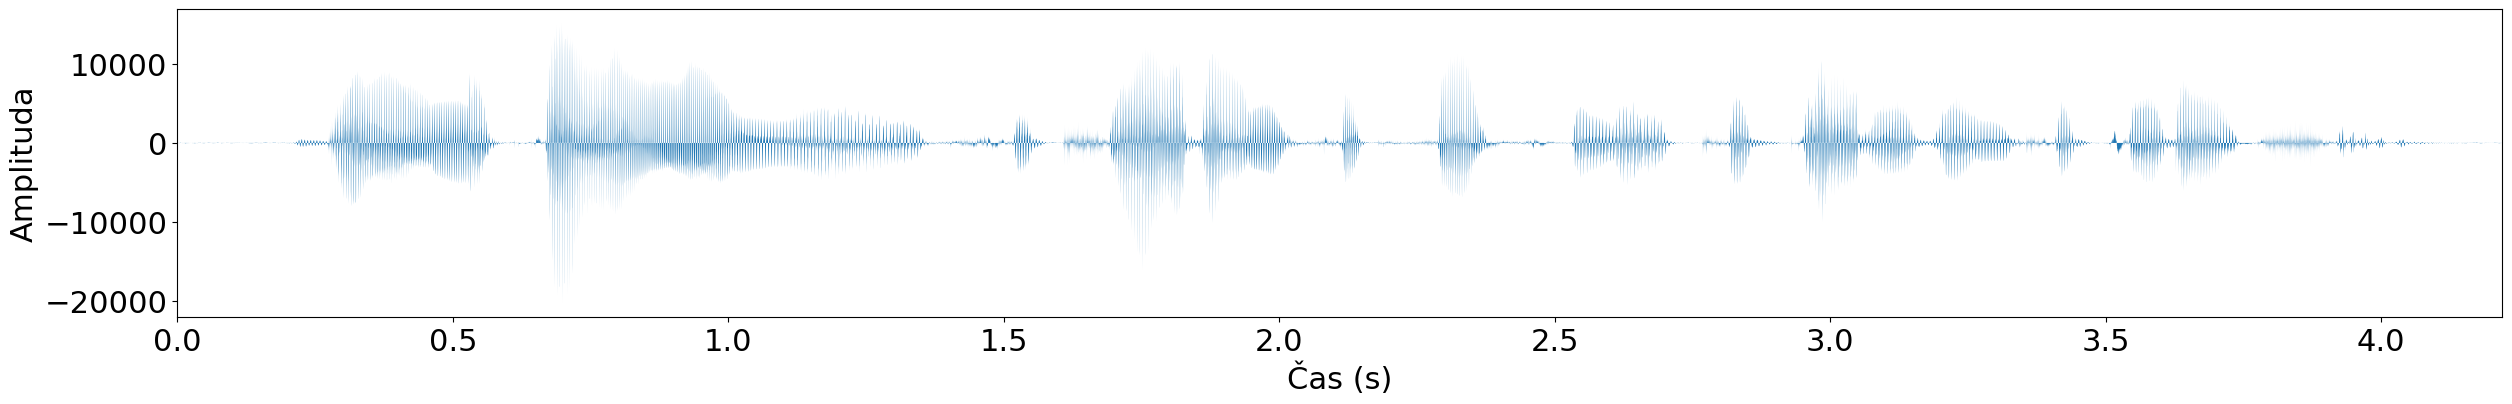
\includegraphics[scale=0.24]{obrazky-figures/s2.png}
    \caption{\label{fig:ref-s2}Druhý mluvčí ze směsi}
\end{figure}

\begin{figure}[H]
    \centering
    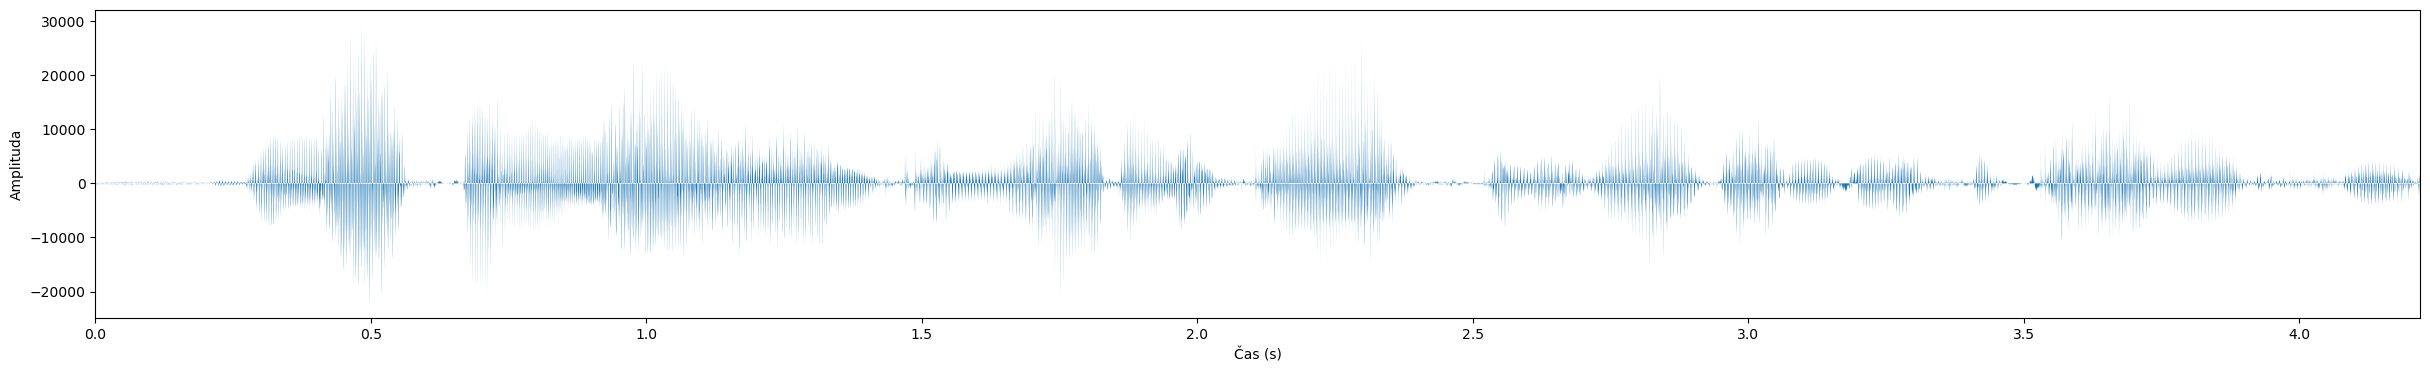
\includegraphics[scale=0.24]{obrazky-figures/mix.png}
    \caption{\label{fig:ref-mixture}Ukázka směsi dvou mluvčích}
\end{figure}

Lze si všimnout, že sečtením signálů jednotlivých mluvčích na obrázku~\ref{fig:ref-s1} a~\ref{fig:ref-s2} dostaneme signál původní směsi~\ref{fig:ref-mixture}.


%------------------------------------------------------------------------------


\section{Průběh trénování}
Bylo natrénováno $7$ modelů s~různými hodnotami zkoumaných hyper--parametrů, jak ukazují tabulky~\ref{tab:vliv-X4},~\ref{tab:vliv-X6} a~\ref{tab:vliv-X8}. Hodnota $X$ představuje počet konvolučních bloků, hodnota $R$ představuje počet opakování sekvence $X$ bloků a hodnota \uv{segment length} představuje počet vzorků v~jednom segmentu. Trénování proběhlo na datasetu Wall Street Journal (WSJ0), který obsahuje $20000$ trénovacích nahrávek následováno průchodem validačního datasetu, který obsahuje $10000$ nahrávek, na konci každé epochy. K~tomu byl použit stroj na Google Colab -- Tesla P100-PCIE, který poskytuje rovněž výkonné GPU. Doba trénování jednotlivých modelů se pohybovala kolem $20$ hodin. Všechny modely byly trénovány po 60 epoch s~hodnotou $\texttt{learning~rate} = 0.001$ a velikostí mini--batchů fixovanou na $50$ segmentů v~jednom mini--batchi. Hodnotu loss během trénování zobrazují, pro vybrané modely, grafy~\ref{graf:X864R4trainloss} a~\ref{graf:X8R4trainlosssegments}. Dále grafy~\ref{graf:X8R4validtrainloss} a~\ref{graf:X4R4validtrainloss} zobrazují trénovací i validační hodnoty loss na konci epoch v~průběhu trénování vybraných modelů.

%\todo{https://www.tablesgenerator.com/}.

\begin{figure}[H]
    \centering
    \begin{minipage}{0.45\textwidth}
        \centering
        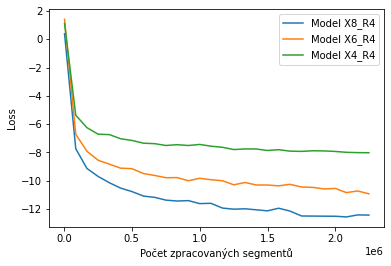
\includegraphics[width=1.0\textwidth]{obrazky-figures/expX864R4trainloss.png}
        \caption{\label{graf:X864R4trainloss}Hodnota loss při trénování modelů s~různým počtem konvolučních bloků. Z~grafu je patrné, že se zmenšujícím se počtem bloků se zhoršuje natrénovaný model.}
    \end{minipage}\hfill
    \begin{minipage}{0.45\textwidth}
        \centering
        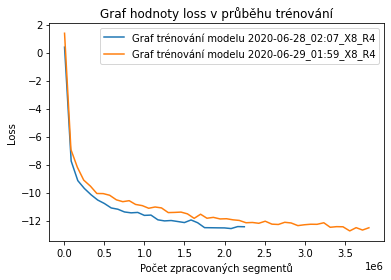
\includegraphics[width=1.0\textwidth]{obrazky-figures/expX8R4trainlosssegments.png}
        \caption{\label{graf:X8R4trainlosssegments}Graf trénování modelů s~rozdílnou délkou segmentů při trénování. Vzhledem k~tomu, že je graf vykreslený v~závislosti na počtu segmentů, tak model, který měl délku segmentů kratší (oranžový graf), tak jich zpracoval více, proto je delší než modrý.}
    \end{minipage}
\end{figure}

\begin{figure}[H]
    \centering
    \begin{minipage}{0.45\textwidth}
        \centering
        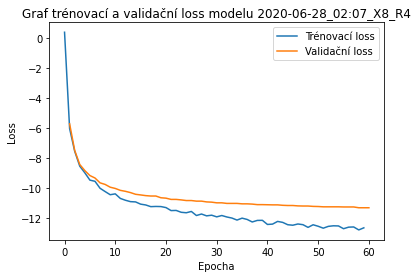
\includegraphics[width=1.0\textwidth]{obrazky-figures/expX8R4validtrainloss.png}
        \caption{\label{graf:X8R4validtrainloss}Graf trénovací a validační loss pro každou epochu trénování. Model má rozměry $X=8$, $R=4$.}
    \end{minipage}\hfill
    \begin{minipage}{0.45\textwidth}
        \centering
        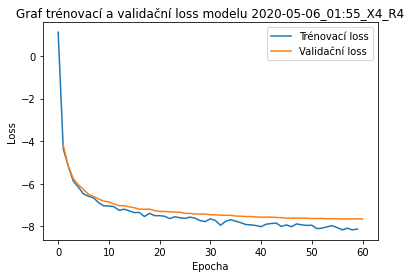
\includegraphics[width=1.0\textwidth]{obrazky-figures/expX4R4validtrainloss.png}
        \caption{\label{graf:X4R4validtrainloss}Graf trénovací a validační loss pro každou epochu trénování. Model má rozměry $X=4$, $R=4$.}
    \end{minipage}
\end{figure}


%------------------------------------------------------------------------------

%\section{Experimenty s~modely}


%---------------------------------------------------------------------------------------------
\section{Vliv parametrů X a R}
\todo{mozna nejake fajnove grafy porovnani vysledky mezi jednotlivymi X, obrazky, grafy pro sdr, pesq, stoi}

Rozměry modelů mají značný vliv na přesnost. V~této části se zaměřím na vliv dvou parametrů -- X a R. Parametr X ovlivňuje počet konvolučních bloků, což přímo ovlivňuje velikost receptive field, což se dá popsat jako velikost kontextu, který síť dokáže vidět. Parametr R udává, kolikrát se sekvence X konvolučních bloků opakuje. Tabulky~\ref{tab:vliv-X8},~\ref{tab:vliv-X6} a~\ref{tab:vliv-X4} přehledně ukazují, jaké modely a o~jakých kombinacích parametrů byly natrénovány.

\begin{table}[!htbp]
\centering
\caption{Tabulka zobrazující vliv počtu opakování pro $X=8$ konvolučních bloků na výsledky testování.}
\label{tab:vliv-X8}
\begin{tabular}{|l|l|l|l|l|l|}
\hline
\textbf{X} & \textbf{R} & \textbf{Délka segmentů {[}vzorky{]}} & \textbf{SDR {[}dB{]}} & \textbf{STOI} & \textbf{PESQ} \\ \hline
8 & 2 & 32000 & 12.71 & 0.94 & 2.71 \\ \hline
8 & 4 & 32000 & 12.45 & 0.93 & 2.69 \\ \hline
\end{tabular}
\end{table}

Modely o~kombinaci parametrů z~tabulky~\ref{tab:vliv-X8} dosahují nejlepších výsledků. Výrazného zlepšení oproti menším modelům s~parametrem dosahují u~metriky SDR hodnoty až $12.71$~dB. Modely si vedou oproti menším poměrně lépe i v~metrice STOI, kde dosahují až hodnoty $2.71$. Podle této tabulky se zdá, že parametr R nemá moc velký vliv na výslednou přesnost sítě. Model s~nižším počtem opakování dokonce dosahuje lehce lepších výsledků než model s~počtem opakování $R = 4$. Důvodem by mohlo být to, že v~závislosti na velikosti trénovaného modelu by mohla lépe vyhovovat menší či větší hodnota \texttt{learning~rate}, než ta, která byla použita při trénování ($0.001$).

\begin{table}[!htbp]
\centering
\caption{Tabulka zobrazující vliv počtu opakování pro $X=6$ konvolučních bloků na výsledky testování.}
\label{tab:vliv-X6}
\begin{tabular}{|l|l|l|l|l|l|}
\hline
\textbf{X} & \textbf{R} & \textbf{Délka segmentů {[}vzorky{]}} & \textbf{SDR {[}dB{]}} & \textbf{STOI} & \textbf{PESQ} \\ \hline
6 & 2 & 32000 & 10.80 & 0.92 & 2.52 \\ \hline
6 & 3 & 32000 & 10.78 & 0.92 & 2.52 \\ \hline
6 & 4 & 32000 & 10.69 & 0.92 & 2.52 \\ \hline
\end{tabular}
\end{table}

\begin{table}[!htbp]
\centering
\caption{Tabulka zobrazující vliv počtu opakování pro $X=4$ konvolučních bloků na výsledky testování.}
\label{tab:vliv-X4}
\begin{tabular}{|l|l|l|l|l|l|}
\hline
\textbf{X} & \textbf{R} & \textbf{Délka segmentů {[}vzorky{]}} & \textbf{SDR {[}dB{]}} & \textbf{STOI} & \textbf{PESQ} \\ \hline
4 & 4 & 32000 & 9.23 & 0.89 & 2.23 \\ \hline
\end{tabular}
\end{table}

Při zmenšování počtu konvolučních bloků X lze vidět znatelný pokles přesnosti ve sledovaných metrikách. Tabulky~\ref{tab:vliv-X6} a~\ref{tab:vliv-X4} obsahují rozměry těchto modelů a jejich dosaženou přesnost. V~první tabulce pro model s~velikostí $X=6$ téměř nedochází k~nějakému znatelnému zvýšení přesnosti při modifikaci parametru R. Znovu se tedy ukazuje, že parametr R nemá velký vliv na celkový výkon sítě. Druhá tabulka ukazuje hodnoty, zmenšíme--li model ještě více. Při parametru $X=4$ má model nejnižší přesnost z~mých natrénovaných modelů ve všech měřených metrikách, z~nichž největšího rozdílu doznaly metriky SDR a PESQ. 

Zdá se, že příčinou, proč má změna parametru X takový vliv na výkon, přímo souvisí s~dilatačním faktorem, který se zvyšuje právě se zvyšujícím se počtem konvolučních bloků.


Přestože víme, že nejlépe si vede model o~rozměrech $X=8$ a $R=2$ s~jeho výslednou hodnotou SDR $12.71$~dB ale tato hodnota nám neříká nic o~výsledcích přesnosti jednotlivých směsí, protože je to průměrná hodnota ze všech nahrávek. Histogram~\ref{fig:sdrhistogram} zobrazuje rozdělení hodnoty SDR v~rámci zpracovaných nahrávek.

\begin{figure}[H]
    \centering
    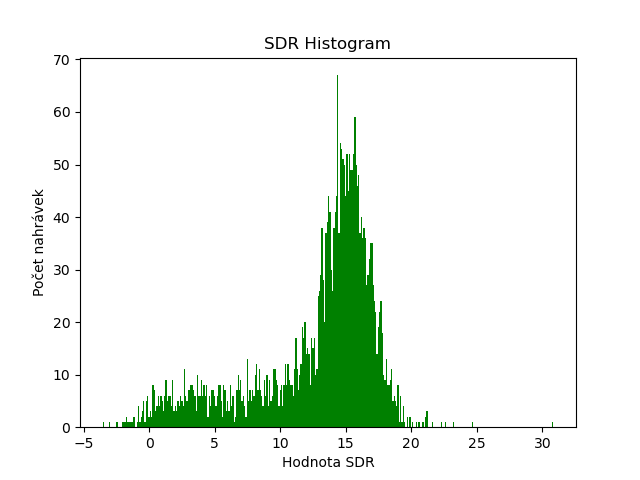
\includegraphics[scale=0.8]{obrazky-figures/sdrhistogramX8R2.png}
    \caption{\label{fig:sdrhistogram}Histogram hodnot SDR pro jednotlivé separace.}
\end{figure}

Na první pohled je vidět největší koncentrace nahrávek kolem hodnoty SDR $15$~dB. Některé nahrávky dokonce  dosáhly hodnoty větší než $19$~dB, což by také příjemně zvyšovalo celkovou přesnost modelu, ale vzhledem k levé části od největší koncentrace je vidět, že pro mnoho nahrávek dosahovala síť pouze přesnosti od $0$~dB po $10$~dB. 


%---------------------------------------------------------------------------------------------
\section{Vliv délky segmentů}
Pro zjištění, zda--li má různá délka segmentů při trénování vliv na přesnost sítě, byly natrénovány dva modely o~stejných rozměrech, jak ukazuje tabulka~\ref{tab:vliv-segment-length}. Jak je vidět, jeden model při trénování segmentoval nahrávky na délku 16000 vzorků, zatímco druhý na 32000 vzorků.

\begin{table}[!htbp]
\centering
\caption{Tabulka zobrazující vliv délky segmentů na výsledky testování.}
\label{tab:vliv-segment-length}
\begin{tabular}{|l|l|l|l|l|l|}
\hline
\textbf{X} & \textbf{R} & \textbf{Délka segmentů {[}vzorky{]}} & \textbf{SDR {[}dB{]}} & \textbf{STOI} & \textbf{PESQ} \\ \hline
8 & 4 & 32000 & 12.45 & 0.93 & 2.69 \\ \hline
8 & 4 & 16000 & 12.49 & 0.93 & 2.7 \\ \hline
\end{tabular}
\end{table}

Testování ukázalo, že model, který používal kratší segmenty, dosahoval zanedbatelně lepších výsledků u~hodnoty SDR ($12.49$~dB), než model, který používal segmenty delší a dosahoval hodnoty SDR $12.45$~dB. Hodnoty ostatních metrik dosahují téměř stejných hodnot v~případě obou modelů.


%---------------------------------------------------------------------------------------------
\section{Úspěšnost s~ohledem na pohlaví mluvčích}
Testovací nahrávky jsou náhodné kombinace mužských a ženských mluvčích. Pro separaci dvou mluvčích tedy mohou vzniknout až 3 typy nahrávek na základě pohlaví mluvčího -- muž--muž, muž--žena a žena--žena. Jednotlivé kombinace mluvčích mohou být pro síť rozdílně náročné pro separaci. Na mém nejlepším modelu o~rozměru $X=8$ a $R=2$ jsem zkoumal, jaké výsledky mají jednotlivé kombinace.

\begin{figure}[H]
    \centering
    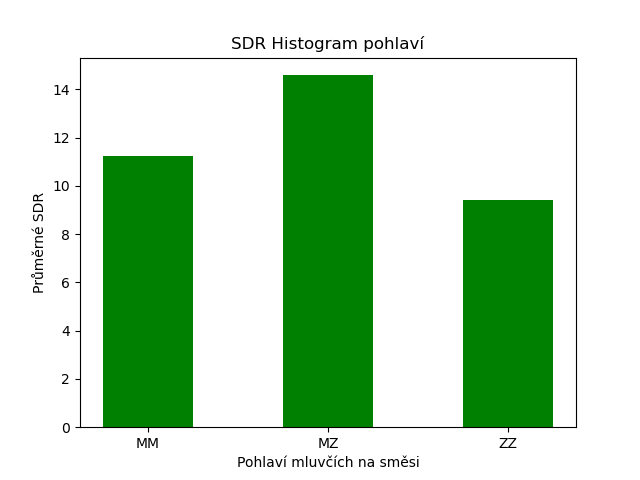
\includegraphics[scale=0.8]{obrazky-figures/sdrpohlaviX8R2.png}
    \caption{\label{fig:sdrpohlavi}Histogram průměrné hodnoty SDR napříč různou kombinací pohlaví. Zkratka \uv{MM} označuje dvojici mužských mluvčích, zkratka \uv{MZ} označuje kombinovanou nahrávku s mužem a ženou a zkratka \uv{ZZ} označuje směs dvou žen.}
\end{figure}

Z~grafu~\ref{fig:sdrpohlavi} lze vypozorovat, jaký vliv má kombinace pohlaví na přesnost sítě. Nejlepších výsledků síť dosahuje v~případě, že na nahrávce jsou zastoupena obě pohlaví. V~takovém případě model dosahuje hodnoty SDR $14.6$~dB. Oproti tomu, v~případě stejných pohlaví si síť vede poměrně hůř. V~případě kombinace dvou žen síť dosahuje hodnoty SDR pouze $9.4$~dB a v~případě kombinace dvou mužů jen o~něco lépe $11.2$~dB. Výsledná hodnota je průměrem hodnot v~dané kombinaci pohlaví.

Výsledkem pozorování je, že síť od sebe separuje mluvčí mnohem lépe v~případě, že jsou zastoupena na směsi rozdílná pohlaví.

%---------------------------------------------------------------------------------------------
%\subsection{MOZNA Vliv hodnoty learning rate}
%\todo{MOZNA ZASE SMAZAT. podkapitola o~rozdilnych LR, jestli stihnu natrenovat jeste - pouze pro X8 R4 --vetsi lr -- mensi loss}

%---------------------------------------------------------------------------------------------
%\subsection{Výsledek inference}
%\todo{podkapitola Inference -- ukazat separovane inferovane nahravky oproti referencni nahravce}



%---------------------------------------------------------------------------------------------
\section{Výsledky referenčního modelu TasNet}
V~referenční studii~\cite{luo2018convtasnet} byly modely trénovány $100$ epoch s~různými hyper--parametry. Já se zaměřím na takové, se kterými experimentuji v~rámci mých modelů. Modely jsou v~nekauzální konfiguraci a používají batch normalizaci (BN).

Nejlepší model ze studie TasNet s~hodnotami parametrů $X=8$ a $R=4$ dosahuje hodnoty $SDR = 14.7$~dB při délce filtrů $L = 20$ vzorků. Hodnoty $SDR = 13.0$~dB dosahuje při hodnotě parametru $X = 7$ a délce filtrů $L = 40$ vzorků. Po zvětšení velikosti filtrů a zmenšení počtu konvolučních bloků (což zmenšuje také hodnotu dilatace) je patrný pokles hodnoty SDR. Při dalším zmenšování modelu dále klesá hodnota SDR, jak zobrazuje tabulka~\ref{tab:tasnet}.

\begin{table}[!htbp]
\centering
\caption{Tabulka ukazující výsledky testovaní referenčních modelů TasNet v~závislosti na konfiguraci.}
\label{tab:tasnet}
\begin{tabular}{|l|l|l|l|l|l|}
\hline
\textbf{L {[}vzorky{]}} & \textbf{X} & \textbf{R} & \textbf{Normalizace} & \textbf{SDR {[}dB{]}} & \textbf{Receptive field {[}s{]}} \\ \hline
20 & 8 & 4 & BN & 14.7 & 2.55 \\ \hline
40 & 7 & 4 & BN & 13.0 & 2.55 \\ \hline
40 & 8 & 2 & BN & 12.6 & 2.56 \\ \hline
40 & 6 & 4 & BN & 12.1 & 1.27 \\ \hline
40 & 7 & 2 & BN & 11.7 & 1.28 \\ \hline
\end{tabular}
\end{table}

Můj nejlepší model v~porovnání s~modely ze studie dosahuje hodnoty SDR $12.71$~dB, jak ukazuje tabulka~\ref{tab:vliv-X8}. Důvodem horší přesnosti může být nedostatečné natrénování modelu (60 epoch oproti jejich 100 epochám), použitá hodnota learning rate při trénování či implementační rozdíly. Přesto tato hodnota ukazuje, že je model již schopen obstojně separovat nahrávky.


%---------------------------------------------------------------------------------------------
\section{Shrnutí výsledků}
\todo{shrnuti a porovnani jednotlivych zmen a vysledku mezi sebou komplexne. Pripadne porovnani vysledku s~ref studii, Okomentovat, co je tedy dulezity parametr, a ktery jde zmensit a neni moc dulezity z~pohledu vysledku evaluace. okomentovat take pohlavi vysledky, prumery sdr, mean, a pod.}


Během testování a experimentů jsem sledoval vliv parametrů X, R a délka segmentů na kvalitu sítě, která je vyhodnocována metrikami SDR, STOI a PESQ. Nejlepších hodnot dosahuje model rozměrově téměř největší (X = 8, R=2), a to SDR $12.71$~dB, STOI $0.94$ a PESQ $2.71$. Při zmenšování hodnoty X se ale přesnost razantně snižuje. Parametr X má tedy dle výsledků největší vliv na přesnost sítě. Oproti tomu změna parametru R přesnost téměř neovlivnila, stejně jako délka segmentů při trénování sítě. Vzhledem k dosaženým přesnostem bych vybral, jako kandidátní, modely o velikosti $R=2$ a $X=8$ nebo $X=6$. Tyto modely dosahují dostatečně dobré kvality separovaných nahrávek.

%Rozdělení hodnoty SDR v rámci jednotlivých separací blah nevim
Graf rozdělení SDR ukázal, že přestože se mnoho hodnot pohybuje lehce pod průměrnou hodnotou SDR daného modelu, tak mnoho separací dosáhlo poměrně větší přesnosti a mnoho separací poměrně menší přesnosti, než je průměrná.

Zajímavý poznatek vyplynul ze sledování hodnoty SDR v rámci ruzných kombinací pohlaví na separovaných nahrávkách. Nejvyšší hodnotu ($14.6$~dB) měly směsi, kde se nacházela dvojice rozdílného pohlaví. Homogenní dvojice dosahovaly mnohem menší přesnosti.


%---------------------------------------------------------------------------------------------
\section{Možná rozšíření a navrhnutá vylepšení}
\todo{k~poslednimu bodu zadani, ze diskutujte -- tak lze jen napsat, ze by mohlo toto toto, proste ukazat, ze jsem se nad tim minimalne zamyslel. mrknout na Tasnet studii, kde to resili jak by to slo vyresit, pripadne jestli bych nasel nejake studie ktere diskutuji o~zlepseni. Kdyz bude cas, tak to pak i vyzkouset a porovnat.}
\todo{Procist studii jaky oni tam navrhuji vylepseni}

%Problémů, které lze v rámci zpracování řeči řešit, je mnoho.
Práce by mohla být rozšířena o variabilnější dataset pro trénování modelů. Zásadní problém při použití mých naučených modelů v reálném scénáři je ten, že trénovací dataset není variabilní, když nepočítám různé kombinace mluvčích. V případě, že by nahrávky řečníků byly pořízeny ve variabilnějším prostředí s rozdílnou technikou, mikrofony a různým ruchem v pozadí (další hlasy, hudba či tleskot), model by tak byl lépe využitelný. Trénování by také mohlo být rozšířeno o nahrávky s větším počtem mluvčích, což by ale vyžadovalo rozsáhlejší implementační úpravy.

Přímo na model by se dalo navázat další neuronovou sítí, která by se učila identifikovat řečníka či analyzovat vlastnosti jeho hlasu a na základě toho provádět další operace. Další možností je přepis separované řeči mluvčích na text. 

%----------------------------------------------------------------------------------------------------------------------------------------------------------------------
%----------------------------------------------------------------------------------------------------------------------------------------------------------------------

\chapter{Závěr}
\label{zaver}
Cílem práce bylo implementovat síť podle architektury TasNet pro separaci mluvčích v~časové doméně a porovnat vliv velikosti sítě na kvalitu separace. Síť byla implementována za pomoci frameworku PyTorch a jazyku Python a natrénována na datasetu obsahujícím jednokanálové směsi dvou mluvčích. Bylo natrénováno $7$ modelů, které se od sebe lišily počtem opakujících se konvolučních bloků, velikostí časové dilatace a délkou vstupních segmentů směsí. Pro účel vyhodnocení modelů byly použity metriky SDR, STOI a PESQ, které se používají pro měření kvality separace. 

Experimenty ukázaly, že během testování nejlépe dopadla síť, která měla 8 konvolučních bloků po 2 opakováních, učena s~délkou vstupních segmentů $L=4$ sekundy. Tento model dosáhl po 60 epochách trénování hodnoty až $12.71$~dB a tím se stal nejúspěšnějším modelem. Při fyzickém poslechu separovaných nahrávek není slyšet téměř žádný náznak druhého mluvčího. Oproti tomu, nejméně přesný model měl pouze 4 konvoluční bloky, 4 opakování a při délce segmentů $L=4$ sekundy dosahoval hodnoty SDR pouze $9.23$~dB. Přestože podmínky pro trénování nebyly ideální, tak bylo natrénováno několik úspěšných modelů.

Zkoušel jsem separovat také nahrávky, které se v datasetu vůbec nenacházely, ale výsledek se nedá hodnotit jako úspěšný, jelikož hraje velkou roli prostředí, mikrofon, šum v~pozadí a další vlivy, na které byla neuronová síť naučena. Tento problém by se dal překonat rozšířením trénovacího datasetu o~větší škálu nahrávek mluvčích, které by byly pořízeny z~různých zařízení a v~různě rušném prostředí.

\todo{co jak dopadlo, vysledky a vyhodnoceni velikosti modelu a jaky byl nejlepsi}
\todo{Doplnit ještě neco eh}

